\documentclass[11pt,a4paper]{article}
\usepackage[T1]{fontenc}
\usepackage{lmodern,microtype}
\usepackage[margin=22mm,headheight=15pt]{geometry}
\usepackage{amsmath,amssymb,mathtools,bm}
\usepackage{graphicx,xcolor,booktabs,tabularx,array,longtable,float}
\usepackage{enumitem,fancyhdr,hyperref,bookmark}
\definecolor{ink}{HTML}{17354C}
\definecolor{teal}{HTML}{087E8B}
\hypersetup{colorlinks=true,linkcolor=ink,urlcolor=teal,pdftitle={Discussion on 20 Oct},pdfauthor={Discussion Series}}
\pagestyle{fancy}\fancyhf{}
\renewcommand{\headrulewidth}{0pt}
\fancyfoot[C]{\thepage}
\setlength{\parindent}{0pt}\setlength{\parskip}{5pt plus 1pt}
\setlength{\emergencystretch}{2em}
\setlist{nosep,topsep=4pt}
\allowdisplaybreaks[2]
\newcommand{\ii}{\mathrm{i}}\newcommand{\dd}{\mathrm{d}}
\newcommand{\ee}{\mathrm{e}}\newcommand{\bn}{\widetilde n}
\newcommand{\avg}[1]{\left\langle #1\right\rangle}
\newcommand{\NA}{\mathrm{NA}}\newcommand{\Rea}{\operatorname{Re}}\newcommand{\Ima}{\operatorname{Im}}
\newcommand{\point}[1]{\begin{quote}\small\color{ink}\textbf{Physical meaning.} #1\end{quote}}
\newcommand{\note}[1]{\begin{quote}\small\textbf{Convention / scope.} #1\end{quote}}
\newcolumntype{Y}{>{\raggedright\arraybackslash}X}
\numberwithin{equation}{section}
\setcounter{tocdepth}{1}
\begin{document}
\begin{center}
{\LARGE\bfseries Discussion on 20 Oct}
\end{center}
\vspace{3mm}

\textbf{Conventions used throughout}\par\smallskip
\begin{tabularx}{\textwidth}{@{}lY@{}}\toprule
Symbol & Meaning\\\midrule
$\ee^{-\ii\omega t}$ & Time dependence; a passive material has $\Ima\bn\geq0$.\\
$\lambda_0$, $k_0$ & Vacuum wavelength and wave number, $k_0=2\pi/\lambda_0=\omega/c$.\\
$\bn=n+\ii\kappa$ & Complex refractive index; EUV notation is $1-\delta+\ii\beta$.\\
$\psi_j=k_{z,j}d_j$ & One-pass complex film phase; distinct from the index decrement $\delta$.\\
$r,t$; $\mathcal R,\mathcal T$ & Complex field coefficients; reflected/transmitted power fractions.\\
$W$ & Real wavefront error in length units; phase error is $k_0W$.\\
$(x_p,y_p)=a(u,v)$ & Physical exit-pupil coordinates; $u=\rho\cos\theta$, $v=\rho\sin\theta$.\\
$(\xi,\eta)$; $h$ & Image displacement from an ideal point; dimensionless object-field coordinate.\\
$Z_n^m$; $c_n^m$ & Unit-mean-square Zernike function; its coefficient in length units.\\\bottomrule
\end{tabularx}

% The interface calculation assumes linear, isotropic, nonmagnetic media and planar layers. The imaging calculation assumes a scalar paraxial field, a clear circular pupil, and a lossless image space (vacuum for the displayed formulas). A full EUV mask calculation can require vector diffraction, patterned sidewalls, and polarization-dependent pupil amplitudes.

\section{Complex optical constants: attenuation and phase}
For a monochromatic plane wave travelling into a homogeneous material,
\begin{align}
E(z,t)&=\Rea\!\left\{E_0\ee^{\ii k_0\bn z}\ee^{-\ii\omega t}\right\},
&\bn&=n+\ii\kappa,\\
\widetilde E(z)&=E_0\underbrace{\ee^{-k_0\kappa z}}_{\text{amplitude decay}}
\underbrace{\ee^{\ii k_0nz}}_{\text{phase accumulation}}.
\end{align}
The intensity of one forward wave in the same homogeneous medium is proportional to $|\widetilde E|^2$, so
\begin{equation}
\boxed{\frac{I(z)}{I(0)}=\ee^{-\alpha z},\qquad
\alpha=2k_0\kappa=\frac{4\pi\kappa}{\lambda_0},\qquad
\ell_I=\frac{1}{\alpha}.}
\end{equation}
The amplitude decay length is $1/(k_0\kappa)=2\ell_I$. These lengths must not be confused.

Relative to an equal geometrical path $d$ in vacuum, the material changes the phase by
\begin{equation}
\Delta\phi_{\rm mat}=k_0(n-1)d.
\end{equation}
In EUV notation, $\bn=1-\delta+\ii\beta$:
\begin{equation}
\frac{\widetilde E_{\rm material}(d)}{\widetilde E_{\rm vacuum}(d)}
=\ee^{-k_0\beta d}\ee^{-\ii k_0\delta d}.
\end{equation}
Thus an absorber is a complex optical element: it attenuates and changes phase. Even when transmission is weak, its interfaces and the underlying reflector affect the reflected complex amplitude.

% \point{A binary black-paint model retains only a real amplitude mask. A local reflective model instead has $r(x,y)=|r(x,y)|\ee^{\ii\phi_r(x,y)}$. Where a scalar local model is adequate, a phase change gives an equivalent wavefront error $\Delta W=\Delta\phi_r/k_0$. At a reflection zero the phase is undefined; an unwrapped phase and a reference are needed elsewhere.}

% The propagation factor alone does not include entry/exit reflections. For oblique propagation through a planar film, use $\ee^{\ii k_zd}$ rather than replacing $z$ by a guessed ray-path length. The conserved transverse wave number and boundary phases are part of the thin-film problem. For a patterned EUV absorber, diffraction couples different transverse components; a stack calculation is only the planar building block.

% \textbf{Illustrative calculation, not a material measurement.} If $\lambda_0=13.5\,\mathrm{nm}$, $\delta=0.05$, $\beta=0.02$, and $d=20\,\mathrm{nm}$, then $I(d)/I(0)=\ee^{-4\pi\beta d/\lambda_0}\simeq0.689$ and $\Delta\phi_{\rm mat}\simeq-0.465\,\mathrm{rad}$. These chosen constants demonstrate the two simultaneous effects; they are not assigned to Mo, Si, or a particular absorber.

\section{Maxwell boundary conditions and single-interface amplitudes}
\subsection{Back to Griffiths: Tangential fields are continuous}
From Griffiths we know,
\begin{equation}
\nabla\times\mathbf E=\ii\omega\mathbf B,
\quad \nabla\times\mathbf H=\mathbf J_f-\ii\omega\mathbf D,
\quad \nabla\cdot\mathbf D=\rho_f,
\quad \nabla\cdot\mathbf B=0.
\end{equation}
Take a rectangular loop of length $L$ tangential to the interface and height $\varepsilon$ normal to it. Faraday's integral law has an electric circulation $(E_{1,\tau}-E_{0,\tau})L+O(\varepsilon)$ and a flux term $O(L\varepsilon)$ for bounded fields. Letting $\varepsilon\to0$ gives equality of the tangential electric fields. Ampere--Maxwell gives the corresponding magnetic relation, except that an imposed surface-current sheet can remain finite. With $\widehat{\mathbf n}$ directed from medium 0 to medium 1,
\begin{equation}
\boxed{\widehat{\mathbf n}\times(\mathbf E_1-\mathbf E_0)=0,
\qquad \widehat{\mathbf n}\times(\mathbf H_1-\mathbf H_0)=\mathbf K_f.}
\label{eq:bc}
\end{equation}
We take $\mathbf K_f=0$. A vanishing pillbox also gives
$\widehat{\mathbf n}\cdot(\mathbf D_1-\mathbf D_0)=\sigma_f$ and
$\widehat{\mathbf n}\cdot(\mathbf B_1-\mathbf B_0)=0$.
Normal $E$ need not be continuous, because the permittivity can jump. These are conditions on \emph{total fields} on each side, not on the incident wave alone.

Using a common fixed tangential electric axis, at the boundary
\begin{equation}
E_i+E_r=E_t,\qquad r=\frac{E_r}{E_i},\quad t=\frac{E_t}{E_i}
\quad\Longrightarrow\quad\boxed{1+r=t.}
\label{eq:Ebc}
\end{equation}
% This is a field-amplitude equation, not an equation for optical powers.

\subsection{Side discovery: reflection and Snell's laws}
At the plane $z=0$, the boundary condition must hold for every $x$ and time:
\begin{equation}
E_i\ee^{\ii k_{x,i}x-\ii\omega_i t}
+E_r\ee^{\ii k_{x,r}x-\ii\omega_r t}
=E_t\ee^{\ii k_{x,t}x-\ii\omega_t t}.
\end{equation}
For a stationary, uniform, linear planar interface, a single incident Fourier component cannot produce a different surface frequency or transverse wave number. Hence
\begin{equation}
\omega_i=\omega_r=\omega_t,\qquad
k_{x,i}=k_{x,r}=k_{x,t},\qquad k_{y,i}=k_{y,r}=k_{y,t}.
\end{equation}
The reflected longitudinal component changes sign in medium 0, giving the familiar equality of reflection and incidence angles. Since $k_x=k_0\bn\sin\theta$, the transmitted component obeys
\begin{equation}
\boxed{\bn_0\sin\theta_0=\bn_1\sin\theta_1.}
\end{equation}
This is Snell's law recovered directly from boundary phase matching: a side discovery of a previously known geometrical result.

% For absorbing materials, a complex angle is an algebraic shorthand. It is safer numerically to compute
% \begin{equation}
% k_{z,j}=\sqrt{k_0^2\bn_j^2-k_\parallel^2}.
% \label{eq:kz}
% \end{equation}
% Choose the passive outgoing branch: $\Ima k_{z,j}\geq0$, and the forward-energy branch in the lossless propagating limit. An evanescent transmitted field has positive imaginary $k_z$ and decays. A grating can change tangential momentum by reciprocal-lattice vectors; the uniform-interface argument does not forbid diffraction at a patterned mask.

\subsection{Why the reflected magnetic field has a minus sign}
For a plane wave, $\nabla\to\ii\mathbf k$ in Faraday's law:
\begin{equation}
\boxed{\mathbf H=\frac{1}{\mu_0\omega}\mathbf k\times\mathbf E.}
\label{eq:kcrossE}
\end{equation}
At normal incidence, $\mathbf k\parallel+\widehat z$ and $\mathbf E\parallel\widehat x$ give $\mathbf H\parallel+\widehat y$. Reversing $\mathbf k$ while retaining the fixed electric axis reverses $\mathbf H$. Define $Y_j$ as the forward-wave ratio of the suitably oriented tangential magnetic field to tangential electric field. Then
\begin{equation}
H_i=Y_0E_i,\qquad H_r=-Y_0E_r,\qquad H_t=Y_1E_t.
\end{equation}
Magnetic continuity therefore gives
\begin{equation}
Y_0E_i-Y_0E_r=Y_1E_t
\quad\Longrightarrow\quad\boxed{Y_0(1-r)=Y_1t.}
\label{eq:Hbc}
\end{equation}
The minus sign expresses the reflected propagation direction; it is not a phenomenological absorption term.

\subsection{Solving for reflection and transmission}
Eliminate $t$ using \eqref{eq:Ebc}:
\begin{align}
Y_0(1-r)&=Y_1(1+r),\\
Y_0-Y_1&=(Y_0+Y_1)r.
\end{align}
Thus
\begin{equation}
\boxed{r_{01}=\frac{Y_0-Y_1}{Y_0+Y_1},\qquad
 t_{01}=1+r_{01}=\frac{2Y_0}{Y_0+Y_1}.}
\label{eq:rt}
\end{equation}
If $Y_0=Y_1$, then $r=0,t=1$: the incident wave already satisfies both boundary conditions. A mismatch generally requires a reflected wave to make both fields match.

\subsection{Secondary identities for the later film sum}
Interchanging the incident and transmitted media, while keeping the same tangential-field convention,
\begin{equation}
r_{10}=\frac{Y_1-Y_0}{Y_0+Y_1}=-r_{01},\qquad
 t_{10}=\frac{2Y_1}{Y_0+Y_1}.
\end{equation}
The product and square satisfy
\begin{align}
t_{01}t_{10}&=\frac{4Y_0Y_1}{(Y_0+Y_1)^2},\\
1-r_{01}^2&=\frac{(Y_0+Y_1)^2-(Y_0-Y_1)^2}{(Y_0+Y_1)^2}
=\frac{4Y_0Y_1}{(Y_0+Y_1)^2}.
\end{align}
Therefore
\begin{equation}
\boxed{r_{10}=-r_{01},\qquad t_{01}t_{10}=1-r_{01}^2.}
\label{eq:identities}
\end{equation}
These are algebraic identities for complex amplitudes. The square is $r^2$, \emph{not} $|r|^2$. They remain valid for complex admittances within the stated interface model.

\subsection{Field coefficients versus power coefficients}
For a forward wave the normal time-averaged energy flux is
$S_z=\tfrac12\Rea(Y)|E_\tau|^2$. With a lossless incident medium and flux evaluated at the interface,
\begin{equation}
\boxed{\mathcal R=|r|^2,\qquad
\mathcal T=\frac{\Rea Y_1}{Y_0}|t|^2.}
\end{equation}
For real positive $Y_0,Y_1$, substitution into \eqref{eq:rt} verifies
$\mathcal R+\mathcal T=[(Y_0-Y_1)^2+4Y_0Y_1]/(Y_0+Y_1)^2=1$.
If medium 1 absorbs, $\mathcal T$ here is the flux entering it, which then decays with depth. In an absorbing incident medium, incident/reflected interference also contributes to net normal flux; the naive identification of a separately normalized $1-\mathcal R$ with net input needs care.

\section{Polarization-specific admittances and Fresnel formulas}
Let the incidence plane be $xz$ and the interface normal be $z$.
The \textbf{vacuum wave impedance} is
\begin{equation}
\boxed{Z_{\rm vac}=\sqrt{\frac{\mu_0}{\epsilon_0}}=\mu_0c}
% =\frac{1}{\epsilon_0c}\simeq376.73\,\Omega.}
\end{equation}
Here $\mu_0$ and $\epsilon_0$ are the vacuum permeability and permittivity, and $c=1/\sqrt{\mu_0\epsilon_0}$ is the speed of light in vacuum. For a travelling plane wave in vacuum, $Z_{\rm vac}$ is the ratio of electric- to magnetic-field amplitudes, $|\mathbf E|/|\mathbf H|$; its reciprocal is the vacuum wave admittance. The polarization-specific $Y$ below instead relates the oriented tangential magnetic field to the tangential electric field, so it also contains the incidence-angle factors.
For nonmagnetic media, $\epsilon=\epsilon_0\bn^2$.

\subsection{s (TE) polarization: derive its admittance}
Here $\mathbf E=(0,E_y,0)$ and $\mathbf k=(k_x,0,k_z)$. From \eqref{eq:kcrossE},
\begin{equation}
\mathbf H=\frac{1}{\mu_0\omega}(-k_zE_y,0,k_xE_y).
\end{equation}
Choose $-H_x$ as the oriented tangential magnetic component of a forward wave. Then
\begin{equation}
\boxed{Y_s=\frac{-H_x}{E_y}=\frac{k_z}{\mu_0\omega}
=\frac{\bn\cos\theta}{Z_{\rm vac}}.}
\end{equation}
A backward wave has $k_z\to-k_z$, giving the required opposite sign.

\subsection{p (TM) polarization: derive its admittance}
Now $\mathbf E=(E_x,0,E_z)$ and $\mathbf H=(0,H_y,0)$. In a homogeneous source-free isotropic medium, $\mathbf k\cdot\mathbf D=0$ gives
\begin{equation}
k_xE_x+k_zE_z=0\quad\Longrightarrow\quad E_z=-\frac{k_x}{k_z}E_x.
\end{equation}
For complex $\mathbf k$, this is a bilinear algebraic transversality condition, not ordinary Euclidean orthogonality to a real ray direction. Substitution gives
\begin{align}
H_y&=\frac{k_zE_x-k_xE_z}{\mu_0\omega}
=\frac{k_z^2+k_x^2}{\mu_0\omega k_z}E_x
=\frac{k_0^2\bn^2}{\mu_0\omega k_z}E_x,\\
Y_p&=\frac{H_y}{E_x}=\frac{\omega\epsilon}{k_z}
=\boxed{\frac{\bn}{Z_{\rm vac}\cos\theta}}.
\end{align}
Here the amplitude is $E_x$, the tangential electric component. Using the full $p$-field amplitude instead changes coefficient formulas.

\subsection{The polarization-specific coefficients}
Insert each admittance in \eqref{eq:rt}. The common $1/Z_{\rm vac}$ cancels:
\begin{align}
r_s&=\frac{\bn_0\cos\theta_0-\bn_1\cos\theta_1}
{\bn_0\cos\theta_0+\bn_1\cos\theta_1},&
t_s&=\frac{2\bn_0\cos\theta_0}
{\bn_0\cos\theta_0+\bn_1\cos\theta_1},\\
r_{p,\tau}&=\frac{\bn_0\cos\theta_1-\bn_1\cos\theta_0}
{\bn_0\cos\theta_1+\bn_1\cos\theta_0},&
t_{p,\tau}&=\frac{2\bn_0\cos\theta_1}
{\bn_0\cos\theta_1+\bn_1\cos\theta_0}.
\end{align}
The $p$ expressions follow by multiplying numerator and denominator of the admittance ratios by $\cos\theta_0\cos\theta_1$. At normal incidence both tangential-field polarizations give
\begin{equation}
r=\frac{\bn_0-\bn_1}{\bn_0+\bn_1},\qquad
 t=\frac{2\bn_0}{\bn_0+\bn_1}.
\end{equation}
For real propagating waves, the commonly used reflected $p$ basis may have a reversed tangential axis. In that convention $r_p^{\rm conventional}=-r_{p,\tau}$ and
$t_p^{\rm full}=(\cos\theta_0/\cos\theta_1)t_{p,\tau}$. This sign difference is a basis choice; it must not be changed halfway through a multilayer sum.

\textbf{A check: Brewster incidence.} For lossless positive indices, $Y_{p,0}=Y_{p,1}$ means $n_0\cos\theta_1=n_1\cos\theta_0$. Combining with Snell's law gives $\tan\theta_B=n_1/n_0$ (for distinct indices). Absorbing media generally have a reflectance minimum rather than an exactly zero real-angle reflection.
\clearpage

\section{A film as a geometric series}
Consider medium $0$, a film $1$ of physical thickness $d_1$, and semi-infinite substrate $2$. Reference the incident and reflected amplitudes at the top surface. The one-pass film factor is
\begin{equation}
p_1=\ee^{\ii\psi_1},\qquad \psi_1=k_{z,1}d_1.
\end{equation}
It includes both phase and attenuation: $|p_1|=\ee^{-\Ima(k_{z,1})d_1}$.
For the returning upward wave $k_z$ and the displacement both reverse sign, so its propagation factor is again $p_1$, not $p_1^{-1}$.

\subsection{List the paths before summing them}
\begin{center}
\begin{tabularx}{\textwidth}{@{}lYl@{}}\toprule
Contribution & Ordered events & Amplitude / incident amplitude\\\midrule
Direct & Reflection at upper boundary & $r_{01}$\\
First return & Enter, descend, reflect, ascend, exit & $t_{01}p_1r_{12}p_1t_{10}$\\
Extra round trip & Reflect internally above, descend, reflect below, ascend & $q=r_{10}r_{12}p_1^2$\\\bottomrule
\end{tabularx}
\end{center}
Every return after the first therefore multiplies the amplitude by another $q$:
\begin{equation}
a_0=t_{01}t_{10}r_{12}p_1^2,\quad
 a_1=a_0q,\quad a_2=a_0q^2,\quad\ldots
\end{equation}
For $|q|<1$ the coherent sum is
\begin{align}
r_{\rm film}&=r_{01}+t_{01}t_{10}r_{12}p_1^2
\sum_{\ell=0}^{\infty}q^\ell\\
&=r_{01}+\frac{t_{01}t_{10}r_{12}\ee^{2\ii\psi_1}}
{1-r_{10}r_{12}\ee^{2\ii\psi_1}}.
\label{eq:filmsum}
\end{align}
The derivation is a sum of fields because the alternative paths are coherent. Summing their separate intensities would discard interference. The series argument uses $|q|<1$; the same rational solution can also be obtained directly from boundary equations, including cases treated by a passive limiting procedure.

\subsection{Use the secondary identities to simplify}
Set $z=\ee^{2\ii\psi_1}$. With \eqref{eq:identities},
\begin{align}
r_{\rm film}
&=r_{01}+\frac{(1-r_{01}^2)r_{12}z}{1+r_{01}r_{12}z}\\
&=\frac{r_{01}+r_{01}^2r_{12}z+r_{12}z-r_{01}^2r_{12}z}
{1+r_{01}r_{12}z}\\
&=\boxed{\frac{r_{01}+r_{12}\ee^{2\ii\psi_1}}
{1+r_{01}r_{12}\ee^{2\ii\psi_1}}}.
\label{eq:film}
\end{align}
The transmitted field at the bottom interface is obtained by the same round trips:
\begin{equation}
\boxed{t_{\rm film}=\frac{t_{01}t_{12}\ee^{\ii\psi_1}}
{1+r_{01}r_{12}\ee^{2\ii\psi_1}}.}
\end{equation}
For lossless exterior media, $\mathcal R=|r_{\rm film}|^2$ and
$\mathcal T=(Y_2/Y_0)|t_{\rm film}|^2$; their deficit is absorption in the film. If the substrate absorbs, $\mathcal T$ denotes flux entering the substrate at its top surface.

\textbf{Limiting checks.} If $r_{12}=0$, then $r_{\rm film}=r_{01}$. If $d_1\to0$, then $(r_{01}+r_{12})/(1+r_{01}r_{12})=r_{02}$: the zero-thickness layer disappears. If the film becomes optically thick and absorbing, $\ee^{2\ii\psi_1}\to0$ and only $r_{01}$ remains. A lossless thick film does not have this latter limit, because its phase keeps oscillating.

\section{Multilayers: replace everything below by an effective reflection}
For two finite films, the order is
\begin{equation}
0\;\longrightarrow\;1\;(d_1)\;\longrightarrow\;2\;(d_2)
\;\longrightarrow\;3\;\text{(substrate)}.
\end{equation}
Seen from medium 1 at the $1|2$ boundary, film 2 and substrate 3 have the effective reflection
\begin{equation}
\Gamma_1=\frac{r_{12}+r_{23}\ee^{2\ii\psi_2}}
{1+r_{12}r_{23}\ee^{2\ii\psi_2}}.
\end{equation}
The same film formula then gives
\begin{equation}
r_{\rm stack}=\frac{r_{01}+\Gamma_1\ee^{2\ii\psi_1}}
{1+r_{01}\Gamma_1\ee^{2\ii\psi_1}}.
\end{equation}
Nothing beneath film 1 needs to be re-expanded path by path. Its entire linear response at the chosen reference plane is already contained in $\Gamma_1$.

For $N$ finite layers and substrate $N+1$, define $\Gamma_j$ as reflection of everything to the right of boundary $j|j+1$, as seen from medium $j$ \emph{at that boundary}. Initialize and recurse:
\begin{equation}
\boxed{\begin{aligned}
\Gamma_N&=r_{N,N+1},\\
\Gamma_j&=\frac{r_{j,j+1}+\Gamma_{j+1}\ee^{2\ii k_{z,j+1}d_{j+1}}}
{1+r_{j,j+1}\Gamma_{j+1}\ee^{2\ii k_{z,j+1}d_{j+1}}},
\quad j=N-1,\ldots,0,\\
r_{\rm stack}&=\Gamma_0.
\end{aligned}}
\label{eq:stack}
\end{equation}
At every step add one upper interface, one layer's propagation, and the effective reflection of the deeper structure. Each denominator accounts for all repeated reflections between the new interface and the deeper stack. Calculate $s$ and $p$ separately with the appropriate admittances and the same conserved $k_\parallel$.

\subsection{Why thickness changes phase as well as reflectance}
For one film write $r=(a+bz)/(1+abz)$, where $a=r_{01}$, $b=r_{12}$, and $z=\ee^{2\ii k_zd}$. Holding optical constants fixed,
\begin{equation}
\frac{\partial r}{\partial d}
=\frac{2\ii k_zbz(1-a^2)}{(1+abz)^2},\qquad
\dd\ln|r|=\Rea\!\left(\frac{\dd r}{r}\right),\quad
\dd\arg r=\Ima\!\left(\frac{\dd r}{r}\right).
\end{equation}
Thus one physical thickness perturbation generally changes both magnitude and phase. This is the connection from multilayer materials to pupil amplitude errors and wavefront errors.

% \textbf{EUV interpretation.} Coherent reinforcement of successive periods roughly suggests $2D\cos\alpha\simeq m\lambda_0$ for period $D$ and incidence angle $\alpha$ from the normal. This Bragg estimate omits complex-index corrections and termination; \eqref{eq:stack} is the planar calculation. The textbook's mask/wafer scaling example gives $D=4(0.725+1)\,\mathrm{nm}=6.9\,\mathrm{nm}$ and $2D\cos6^\circ\simeq13.724\,\mathrm{nm}$. It is a scale check, not an exact recovered coating prescription.

A finite patterned absorber also has lateral edges and angular coupling. The geometrical shadow scale $h_{\rm abs}\tan\alpha$ helps explain sensitivity but does not by itself predict printed placement. A rigorous image requires complex diffraction-order amplitudes, the projection pupil, source averaging, and an image/resist metric.
\clearpage

\section{From pupil field to image field}
\subsection{A pupil map is not an image}
Let $A(x_p,y_p)$ be the real nonnegative pupil amplitude and $W(x_p,y_p)$ the residual optical path difference from an ideal converging reference wave. For an image point a distance $f$ away, the paraxial exit-pupil field is
\begin{equation}
U_p(x_p,y_p)=A(x_p,y_p)
\exp\!\left[-\frac{\ii k_0}{2f}(x_p^2+y_p^2)\right]
\exp[\ii k_0W(x_p,y_p)].
\end{equation}
The quadratic phase is the ideal convergence. The residual $W$ measures departures from that reference, not the physical height of a wafer surface.

Fresnel propagation to the reference image plane gives
\begin{align}
U_f(\xi,\eta)&=\frac{\ee^{\ii k_0f}}{\ii\lambda_0 f}
\iint U_p(x_p,y_p)
\exp\!\left[\frac{\ii k_0}{2f}\big((\xi-x_p)^2+(\eta-y_p)^2\big)\right]
\dd x_p\dd y_p.\nonumber
\end{align}
Expand the squares. The pupil-quadratic terms cancel; the remaining image-quadratic phase has unit magnitude and does not affect intensity:
\begin{equation}
\boxed{U_f(\xi,\eta)=C(\xi,\eta)
\iint A\ee^{\ii k_0W}
\ee^{-\ii k_0(x_p\xi+y_p\eta)/f}\dd x_p\dd y_p,}
\label{eq:fourier}
\end{equation}
where $C=\ee^{\ii k_0f}\ee^{\ii k_0(\xi^2+\eta^2)/(2f)}/(\ii\lambda_0 f)$.
With $(x_p,y_p)=a(u,v)$ and $s_x=\NA\xi/\lambda_0$, $s_y=\NA\eta/\lambda_0$, $\NA\simeq a/f$ in vacuum,
\begin{equation}
U_f\propto\int_{u^2+v^2\leq1}A(u,v)\ee^{\ii2\pi W/\lambda_0}
\ee^{-\ii2\pi(us_x+vs_y)}\dd u\dd v,\qquad
I_f\propto|U_f|^2.
\label{eq:fft}
\end{equation}
% \point{The map displays a phase error indexed by pupil position. The image is the interference of contributions from the \emph{whole} pupil. A red lobe in a pupil map is not a red or bright lobe at the same position in the image.}

For $W=0$ and $A=1$ on a disk, angular integration gives
$\int_0^{2\pi}\ee^{-\ii2\pi s\rho\cos\theta}\dd\theta=2\pi J_0(2\pi s\rho)$, and the radial integral gives the normalized amplitude
\begin{equation}
\frac{U_f(s)}{U_f(0)}=\frac{2J_1(2\pi s)}{2\pi s},\qquad
I_f(s)/I_f(0)=\left[\frac{2J_1(2\pi s)}{2\pi s}\right]^2.
\end{equation}
Its first dark ring is at $s\simeq0.610$, or image radius $0.610\lambda_0/\NA$.

\subsection{Wavefront slopes give ray displacements}
The local phase and its gradients are
\begin{align}
\Phi(x_p,y_p)&=-\frac{k_0}{2f}(x_p^2+y_p^2)+k_0W(x_p,y_p),\\
\frac{k_x}{k_0}&=-\frac{x_p}{f}+\frac{\partial W}{\partial x_p},&
\frac{k_y}{k_0}&=-\frac{y_p}{f}+\frac{\partial W}{\partial y_p}.
\end{align}
For small ray angles, propagation over $f$ produces
\begin{equation}
\xi\simeq x_p+f\frac{k_x}{k_0}
=x_p-x_p+f\frac{\partial W}{\partial x_p},
\end{equation}
and similarly for $\eta$. Therefore
\begin{equation}
\boxed{(\xi,\eta)=f\nabla_pW
=\frac{f}{a}\left(\frac{\partial W}{\partial u},\frac{\partial W}{\partial v}\right).}
\label{eq:rays}
\end{equation}
The same result follows by stationary phase in \eqref{eq:fourier}:
$\partial_{x_p}(W-x_p\xi/f-y_p\eta/f)=0$.
Thus the ray relation and diffraction integral agree under the same sign convention. Rays describe local phase directions; diffraction determines the finite intensity distribution, including interference and the Airy scale.

% \note{In a lossless image medium of index $n_i$, retain phase error $k_0W$, but replace the ideal propagation wave number by $n_i k_0$. Then $(\xi,\eta)=(f/(n_i a))\nabla_{u,v}W$, and $\NA\simeq n_i a/f$. The vacuum formulas are adequate for this teaching model.}

\subsection{Piston and tilt: two exact field results}
For piston $W=p$, \eqref{eq:fourier} simply acquires $\ee^{\ii k_0p}$, so intensity is unchanged everywhere. Likewise \eqref{eq:rays} gives zero ray displacement. Global piston cannot be recovered from an intensity-only image of this isolated field; an external coherent reference would change the measurement.

For tilt $W=t_xu+t_yv$, combine the linear phases in \eqref{eq:fft}:
\begin{equation}
\boxed{I_f(\xi,\eta)=I_0\!\left(\xi-\frac{f}{a}t_x,
\eta-\frac{f}{a}t_y\right),\qquad
\Delta\mathbf x=\frac{f}{a}(t_x,t_y).}
\label{eq:tiltphysical}
\end{equation}
An irrelevant unit-modulus image phase may differ between the corresponding complex fields. All pupil rays receive the same displacement. Shape is unchanged, while placement is changed. Recentring an image removes this placement information; a tilt-removed RMS cannot bound the removed shift.

\textbf{Reconciliation with textbook \S6.4.} That section uses a \emph{spatial-frequency pupil} with the inverse Fourier kernel $\ee^{+\ii2\pi\boldsymbol\nu\cdot\mathbf x}$. It consequently writes $\Delta\mathbf x=-\mathbf t_{\rm freq}/\NA$. Equation \eqref{eq:fourier} uses the physical pupil with the negative kernel. Identifying $\boldsymbol\nu=-(x_p,y_p)/(\lambda_0 f)$ reverses the normalized pupil axes, so $\mathbf t_{\rm freq}=-\mathbf t$. The physical predictions agree. The HTML and plots use the positive displacement in \eqref{eq:tiltphysical}.

\subsection{Defocus: change the observation plane}
At $z=f+\Delta z$, expand $1/z\simeq1/f-\Delta z/f^2$. After combining propagation and ideal lens phases, the added residual OPD is
\begin{equation}
W_{\rm focus}=-\frac{\Delta z}{2f^2}(x_p^2+y_p^2)
=-\frac{a^2\Delta z}{2f^2}\rho^2.
\label{eq:focus}
\end{equation}
Equivalently, combining $W=d\rho^2$ with the ideal focusing phase gives $1/f_{\rm new}=1/f-2d/a^2$. At leading order, this pupil error is compensated by
\begin{equation}
\Delta z=\frac{2f^2d}{a^2},\qquad
(\xi,\eta)_{z=f}=\frac{2fd}{a}(u,v).
\end{equation}
The ray spot at the original plane is a disk for a uniformly filled pupil. A common change of focus can remove defocus; it cannot remove all higher-order shapes. Best-focus and fixed-plane results therefore answer different questions.

\section{Deriving the five third-order aberration families}
\subsection{Why these terms occur}
For a centred, rotationally symmetric system let the normalized field vector be $\mathbf h$ and pupil vector $\mathbf u=(u,v)$. Reflection-symmetric scalar polynomials can be built from $\mathbf u^2$, $\mathbf h^2$, and $\mathbf h\cdot\mathbf u$. Once the paraxial reference is chosen, the lowest classical residual wave terms have total degree four. The independent pupil-dependent terms are
$(\mathbf u^2)^2$, $\mathbf u^2(\mathbf h\cdot\mathbf u)$,
$(\mathbf h\cdot\mathbf u)^2$, $\mathbf h^2\mathbf u^2$, and
$\mathbf h^2(\mathbf h\cdot\mathbf u)$. A pure $\mathbf h^4$ term is pupil-constant piston.

Choose the field along $x$, $\mathbf h=(h,0)$, and set $\rho^2=u^2+v^2$:
\begin{equation}
\boxed{W=A\rho^4+Bh\,u\rho^2+Ch^2u^2+Dh^2\rho^2+Eh^3u.}
\label{eq:seidel}
\end{equation}
Here $A,\ldots,E$ have length units; numerical factors are absorbed into their definitions. These are the classical Seidel families. They are fourth degree in the wave expansion but give \emph{third-order ray errors} after a pupil derivative. \textbf{These five forms are consequences of geometrical symmetry, not a universal list of all possible wavefront errors.} Centring, axial rotational symmetry, and reflection symmetry restrict the allowed invariants. Off-axis geometries, decentring, tilt/misalignment, non-axisymmetric surfaces, or other broken symmetries can allow additional terms and different field dependencies. The scalar Fourier integral and wavefront-gradient relation do not require that five-term classification; their own paraxial/scalar assumptions still apply.

\subsection{Spherical aberration: a pupil-radius-dependent focus}
For $W=A(u^2+v^2)^2$, differentiate explicitly:
\begin{equation}
\frac{\partial W}{\partial u}=4Au(u^2+v^2),\qquad
\frac{\partial W}{\partial v}=4Av(u^2+v^2).
\end{equation}
Equation \eqref{eq:rays} gives
\begin{equation}
(\xi,\eta)=\frac{4fA}{a}\rho^2(u,v),\qquad
r_{\rm spot}=\frac{4f|A|}{a}\rho^3.
\end{equation}
The ideal reference sphere has already been subtracted; the quartic here is residual error, not the ideal sphere itself. All rays on a pupil annulus have the same radial displacement; marginal rays deviate most. The radial direction after the pupil is
$\theta_r\simeq-a\rho/f+4A\rho^3/a$. Its axial intercept is
\begin{equation}
z_{\rm axis}\simeq\frac{f}{1-4fA\rho^2/a^2}
\simeq f+\frac{4f^2A}{a^2}\rho^2.
\end{equation}
The focal position depends on pupil radius. One defocus adjustment changes all radii together and cannot make this quartic term vanish. Adding defocus to minimize RMS produces balanced spherical aberration, derived below in the Zernike section.

\subsection{Coma: displaced annular ray circles}
Write $b=Bh$. Then $W=bu(u^2+v^2)=b(u^3+uv^2)$, hence
\begin{equation}
\boxed{(\xi,\eta)=\frac{fb}{a}(3u^2+v^2,\,2uv).}
\end{equation}
On a fixed pupil annulus $u=\rho\cos\theta$, $v=\rho\sin\theta$,
\begin{equation}
(\xi,\eta)=\frac{fb\rho^2}{a}(2+\cos2\theta,\,\sin2\theta).
\end{equation}
Opposite pupil points $(u,v)$ and $(-u,-v)$ have identical coma displacement because both derivatives are even under this inversion. Unlike tilt, however, the displacement varies over the pupil, so recentering cannot remove its blur. Each annulus maps to a circle of radius $|fb|\rho^2/a$ centred at
$(2fb\rho^2/a,0)$. Both radius and offset grow with $\rho^2$, producing the asymmetric family of intercepts associated with coma. Diffraction turns this geometrical tendency into a lopsided point image; it is not obtained by colouring these circles as a pupil map.

Balanced Zernike coma subtracts a tilt component from this monomial. That balances its pupil inner product with tilt; it does \emph{not} guarantee that every ray-centroid or peak-position definition vanishes.

\subsection{Astigmatism: two directional foci}
Take $W=c u^2$ with $c=Ch^2$. At the nominal plane,
\begin{equation}
(\xi,\eta)=\frac{2fc}{a}(u,0).
\end{equation}
The pupil collapses geometrically to a line in this particular reference plane. To see the two foci, retain the accompanying isotropic term $d\rho^2$, $d=Dh^2$:
\begin{equation}
W=(c+d)u^2+dv^2,
\qquad
\begin{cases}
\Delta z_x=2f^2(c+d)/a^2,\\
\Delta z_y=2f^2d/a^2.
\end{cases}
\end{equation}
At $\Delta z_x$, the $x$ dependence is focused and the remaining ray line lies along $y$; at $\Delta z_y$, the line lies along $x$. At their midpoint, the effective pupil error is
\begin{equation}
W_{\rm mid}=\frac c2(u^2-v^2)=\frac c2\rho^2\cos2\theta,
\qquad (\xi,\eta)=\frac{fc}{a}(u,-v).
\end{equation}
The ray footprint there is circular for a circular pupil, even though the wavefront is astigmatic. This is a particularly useful warning against reading image shape directly from the pupil map. The two directional focal planes still differ.

\subsection{Field curvature: best focus depends on field position}
For $W=Dh^2\rho^2$,
\begin{equation}
(\xi,\eta)=\frac{2fDh^2}{a}(u,v),\qquad
\Delta z_{\rm best}(h)=\frac{2f^2Dh^2}{a^2}.
\end{equation}
At any one field point this is simply defocus. Its distinguishing feature is the $h^2$ dependence across the field. A curved focal surface can have locally sharp images while a flat wafer is out of focus away from the centre.

The raw astigmatic term contains an isotropic part:
\begin{equation}
Ch^2u^2=\frac{Ch^2}{2}\rho^2\cos2\theta+\frac{Ch^2}{2}\rho^2.
\end{equation}
Consequently the mean focal surface in \eqref{eq:seidel} depends on $(D+C/2)h^2$. Separating field curvature from astigmatism must respect the chosen coefficient convention.

\subsection{Distortion: field-dependent placement without local blur}
For $W=Eh^3u$,
\begin{equation}
\boxed{(\xi,\eta)=\left(\frac{fE}{a}h^3,0\right).}
\end{equation}
Every pupil point receives the same displacement: locally it is pure tilt, and the point-spread shape is preserved. Across field points it is a nonlinear placement law. If the ideal image height is $H=H_*h$, then
$H_{\rm actual}=H+(fE/(aH_*^3))H^3$. This changes magnification with field, bending a grid even when each local point is sharp. Barrel/pincushion terminology depends on the signed mapping; state that mapping instead of inferring a sign from a pupil plot.

\subsection{Pupil wavefront maps differently to image field point}
The field coordinate labels the \emph{intended image point}, while $(\xi,\eta)$ describes displacement relative to that point. Each intended point has its own ray bundle and reference sphere. Its bundle can encounter different parts of the surfaces at different angles, so
\begin{equation}
W=W(\rho,\theta;\mathbf h),\qquad
W(\rho,\theta;\mathbf h)=\sum_{n,m}c_n^m(\mathbf h)Z_n^m(\rho,\theta).
\end{equation}
Time and thermal state can add further dependencies. In the classical centred expansion, coma varies as $h$, astigmatism/field defocus as $h^2$, and distortion as $h^3$. An off-axis multi-mirror projector need not obey these restrictions. One local pupil measurement cannot establish the field dependence.

\subsection{Piston invariance for any linear propagation kernel}
The result does not require the Fresnel approximation. If
$U_W(q)=\int K(q,p)A(p)\ee^{\ii k_0W(p)}\dd p$, then for a real constant $c_0$,
\begin{align}
U_{W+c_0}(q)&=\int K(q,p)A(p)\ee^{\ii k_0W(p)}\ee^{\ii k_0c_0}\dd p
=\ee^{\ii k_0c_0}U_W(q),\\
I_{W+c_0}(q)&=|\ee^{\ii k_0c_0}|^2I_W(q)=I_W(q).
\end{align}
Every relative phase $k_0[W(p_1)-W(p_2)]$ is preserved. Each coherent source contribution retains its intensity before a partially coherent sum, so intensity-derived CD, pattern shift, and process-variation bands also remain unchanged. A phase change on only one pupil segment or one interferometer arm is a relative phase, not this global piston.

\subsection{Compact derivative table}
\begin{center}\small
\begin{tabularx}{\textwidth}{@{}l l Y@{}}\toprule
Family & $W$ & $(a/f)(\xi,\eta)=\nabla W$\\\midrule
Piston & $p$ & $(0,0)$\\
Tilt & $t_xu+t_yv$ & $(t_x,t_y)$\\
Defocus & $d\rho^2$ & $2d(u,v)$\\
Spherical & $A\rho^4$ & $4A\rho^2(u,v)$\\
Coma & $Bh\,u\rho^2$ & $Bh(3u^2+v^2,2uv)$\\
Astigmatism, raw & $Ch^2u^2$ & $2Ch^2(u,0)$\\
Field curvature & $Dh^2\rho^2$ & $2Dh^2(u,v)$\\
Distortion & $Eh^3u$ & $(Eh^3,0)$\\\bottomrule
\end{tabularx}\end{center}

% \section{Visual bridge: pupil map, rays, and diffraction image}
% The following comparison uses unit-RMS Zernike modes with a common coefficient $c/\lambda_0=0.15$. This value is chosen to make differences visible, not as a small-error design specification. For each row, $W=cZ$, the middle panel uses \eqref{eq:rays}, and the right panel uses \eqref{eq:fft}. The geometrical image coordinate is $\mathbf s_{\rm ray}=\nabla_{u,v}(W/\lambda_0)$. All diffraction panels use the \emph{same ideal-peak intensity normalization}; individual peaks have not been rescaled to one.

% The companion \href{run:aberration_explorer.html}{\texttt{aberration\_explorer.html}} provides selectable modes, signed coefficient, added defocus, and linear/log intensity display. The recovered original chat illustration is also available as \href{run:aberration_illustration.html}{\texttt{aberration\_illustration.html}}, preserving its stored optical data and adding explicit polar and Zernike expressions for every case. Both this figure and the explorer show coherent point images, not a complete partially coherent contact-layer lithography simulation.
% \begin{figure}[H]\centering
% 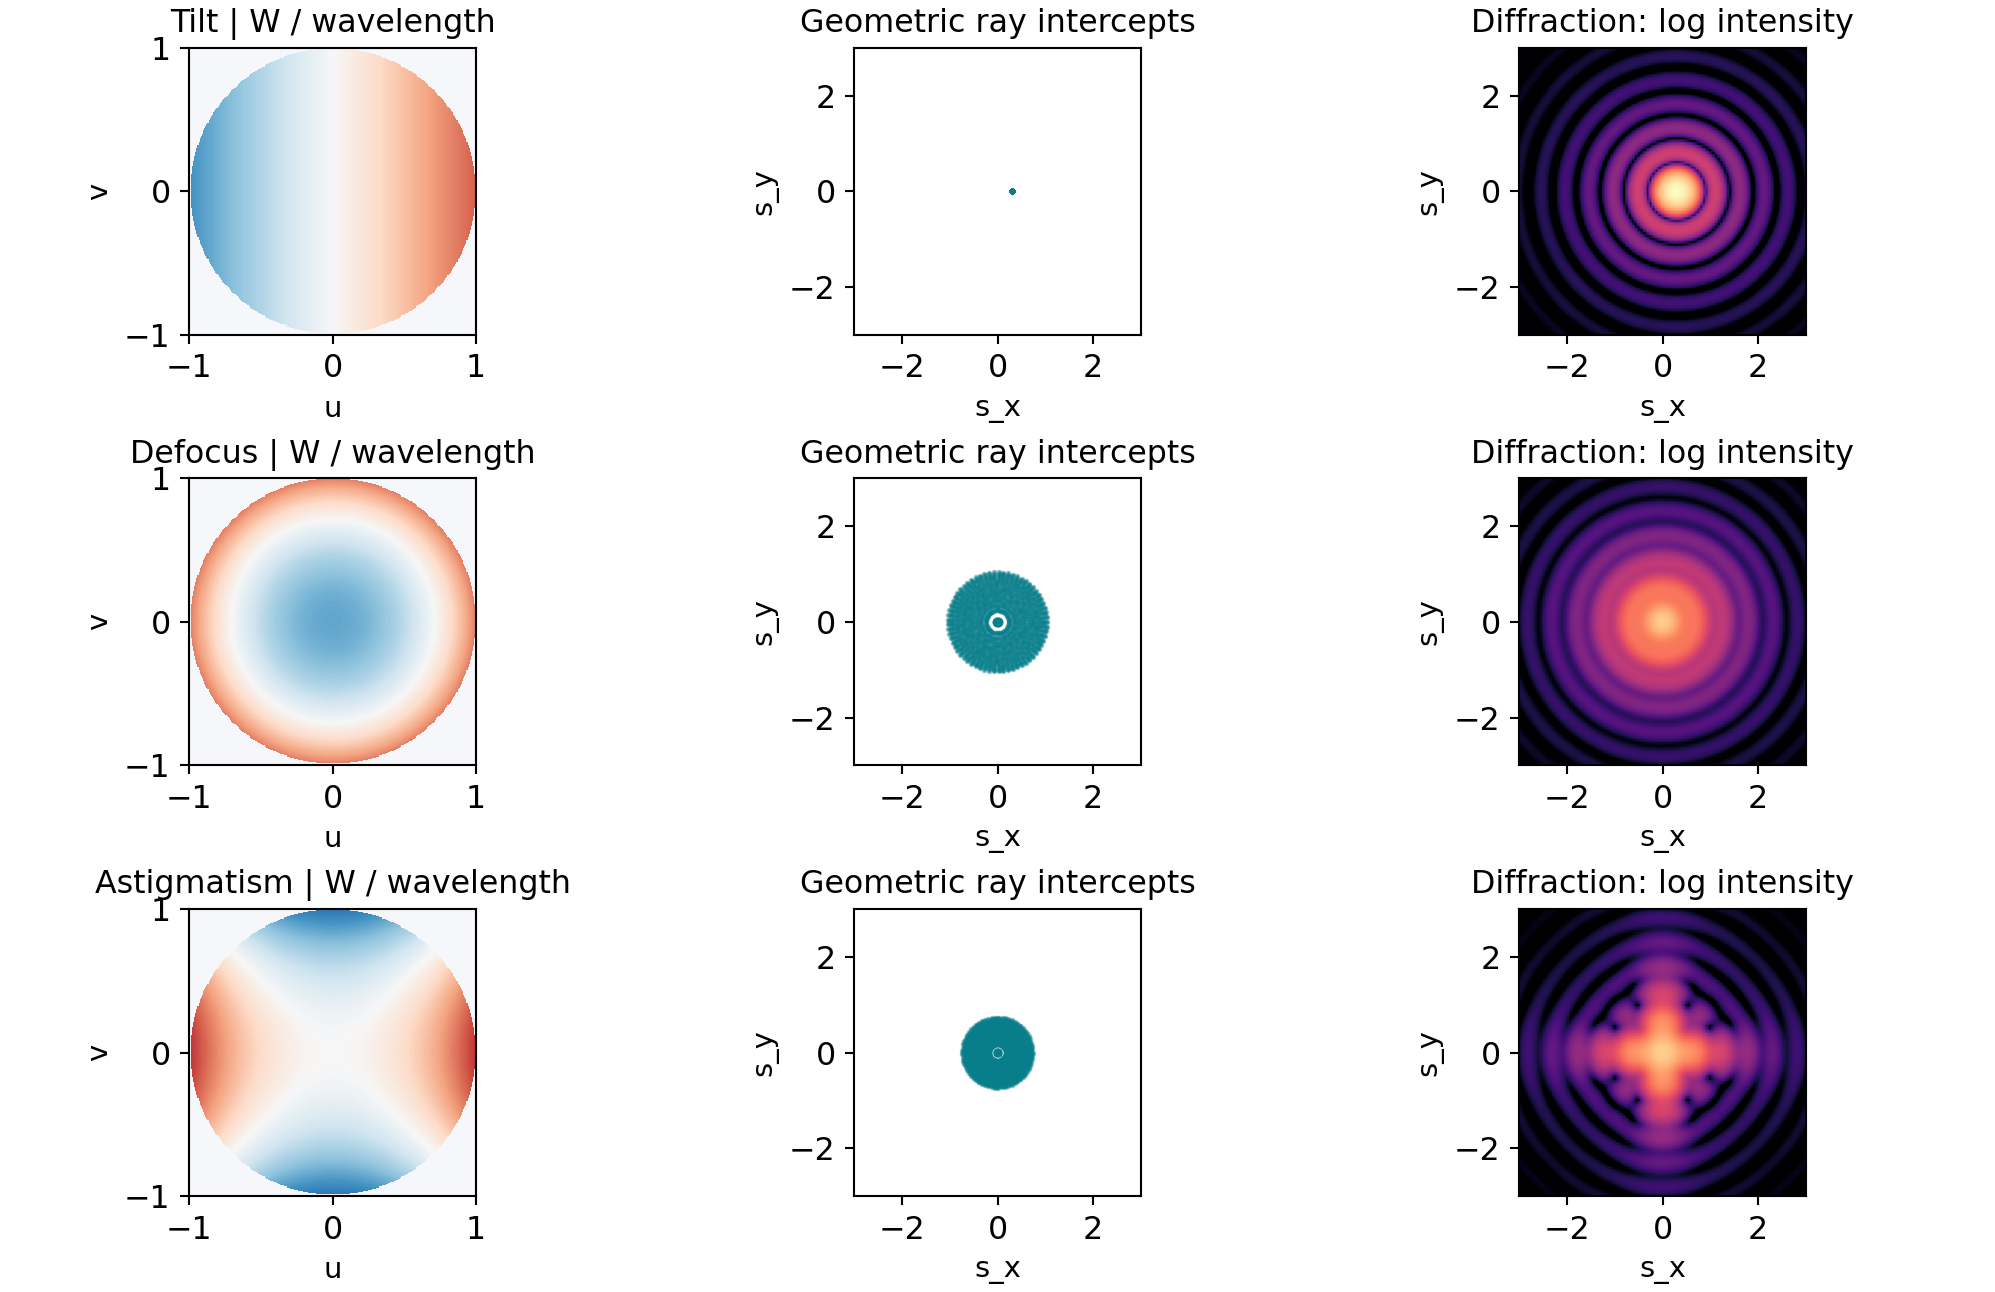
\includegraphics[width=.98\textwidth]{figures/pupil_ray_psf_1.png}
% \caption{Tilt, defocus, and astigmatism at the same coefficient $c/\lambda_0=0.15$. OPD colours share a $[-0.5,0.5]$-wave scale. Ray intercepts have no diffraction width. Intensities use a common logarithmic scale from $10^{-4}$ to one ideal peak. Image axes are $s_x=\NA\xi/\lambda_0$, $s_y=\NA\eta/\lambda_0$.}
% \label{fig:bridge}
% \end{figure}
% \begin{figure}[H]\centering
% 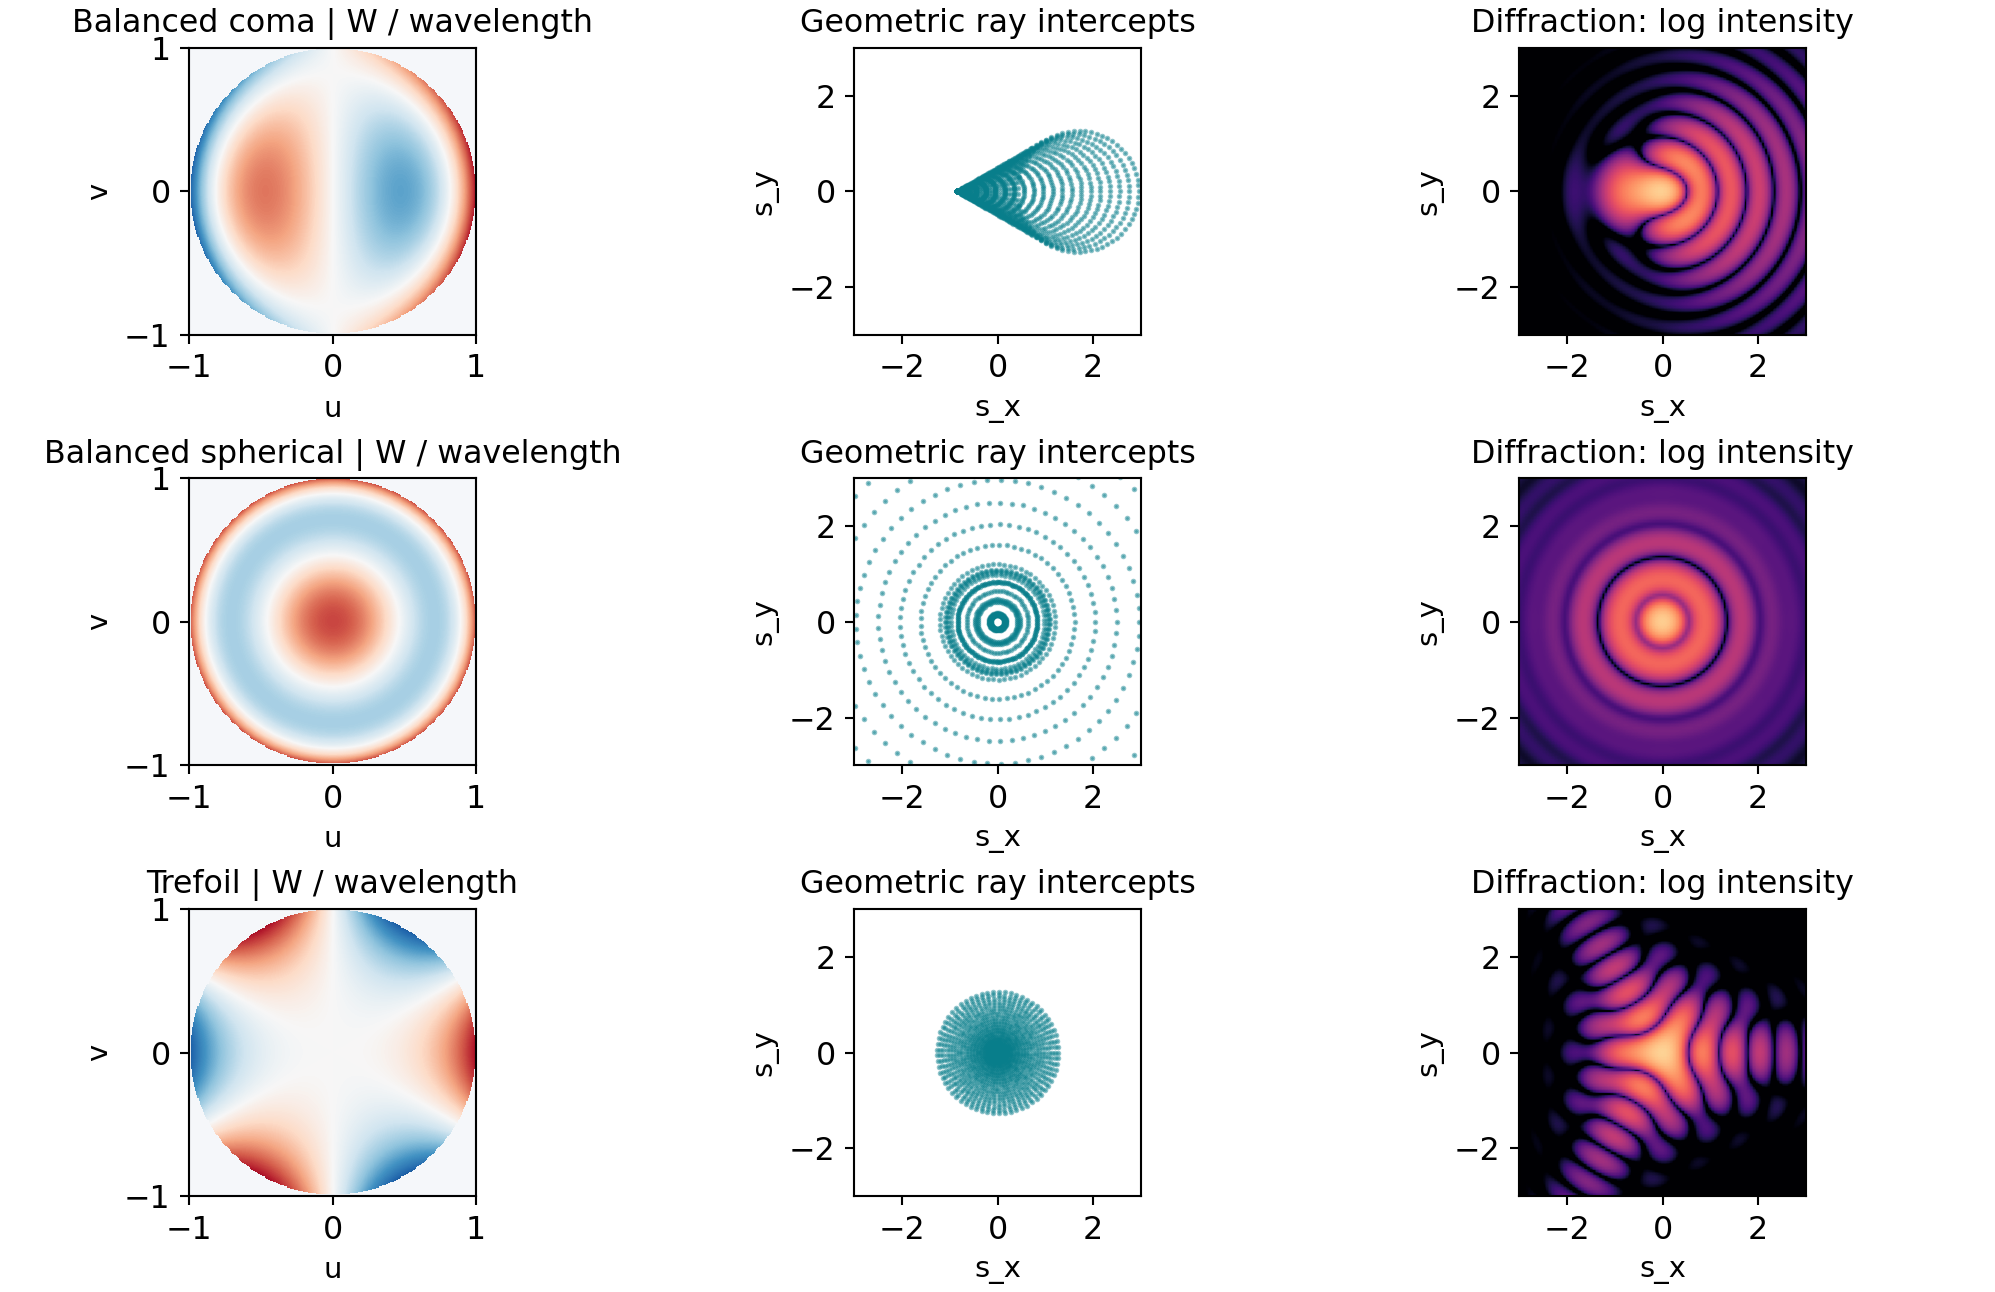
\includegraphics[width=.98\textwidth]{figures/pupil_ray_psf_2.png}
% \caption{Balanced coma, balanced spherical aberration, and trefoil, using exactly the same coefficient, OPD colour limits, image coordinates, and intensity normalization as Fig.~\ref{fig:bridge}. The lower-order balance changes the slopes; the diffraction law is unchanged.}
% \end{figure}

\section{Small-error RMS: useful, but not sufficient}
For a uniform disk pupil at the reference image point, normalize the field by its unaberrated value:
\begin{equation}
\frac{U(0)}{U_0(0)}=\avg{\ee^{\ii\phi}},\qquad
\phi=\frac{2\pi W}{\lambda_0},\qquad
\avg{g}=\frac1\pi\int_0^{2\pi}\int_0^1g\rho\dd\rho\dd\theta.
\end{equation}
Expanding the exponential and retaining intensity terms through second order,
\begin{align}
\avg{\ee^{\ii\phi}}&\simeq1+\ii\avg\phi-\tfrac12\avg{\phi^2},\\
S_{\rm ref}&=\left|\avg{\ee^{\ii\phi}}\right|^2
\simeq1-\avg{\phi^2}+\avg\phi^2
=\boxed{1-\left(\frac{2\pi\sigma_W}{\lambda_0}\right)^2}.
\end{align}
Here $\sigma_W^2=\avg{(W-\avg W)^2}$. The widely used exponential
$S\simeq\exp[-(2\pi\sigma_W/\lambda_0)^2]$ has the same leading term, but is not an exact formula for arbitrary deterministic aberration. At $\sigma_W=\lambda_0/50$, it gives $S\simeq0.9843$.

\textbf{Three distinct ambiguities.}
\begin{enumerate}
\item \textbf{RMS degeneracy.} Many coefficient vectors have the same sum of squares. Equal RMS does not specify mode, orientation, placement, or a pattern's phase differences. Tilt can preserve the peak while shifting it; coma and astigmatism redistribute intensity differently.
\item \textbf{Measurement invariance.} Piston gives exactly the same intensity. If images are recentered, pure tilt also disappears from the retained data. For a real centrosymmetric pupil and even $W$, $U_{-W}(\mathbf s)=U_W^*(-\mathbf s)$ and $U_W(-\mathbf s)=U_W(\mathbf s)$, so a single in-focus point intensity cannot distinguish $W$ from $-W$. Additional planes or references can supply missing information.
\item \textbf{Metric compression.} Different images or wavefronts may share the same few CD, placement, or process-window metrics. Orthogonal pupil coordinates do not guarantee a unique inverse map from these observables.
\end{enumerate}
Strehl normally compares consistent \emph{peak} intensities. The displayed expansion first evaluates a fixed reference point; specify whether tilt or focus has been optimized. With nonuniform amplitude $A$, the coherent field average is weighted by $A$, not automatically by intensity $A^2$. The clear-disk RMS formula cannot be transferred silently to an obscured or apodized pupil.


\section{Zernike modes: orthogonal coordinates on a pupil disk}
\subsection{Introduction to the map atlas}
A Zernike map plots a \emph{basis function on the pupil}, not image brightness. In Fig.~\ref{fig:atlas}, each disk has normalized radius one; horizontal and vertical axes are $u$ and $v$. Colours encode the signed dimensionless value of $Z_n^m$, with the \emph{same colour scale in every panel}. Multiplying a map by coefficient $c_n^m$ gives that mode's wavefront error in length units. The associated phase is $2\pi c_n^mZ_n^m/\lambda_0$.

The two indices have different roles: $n$ is radial polynomial degree, and $|m|$ counts the angular frequency. Positive $m$ denotes a cosine, negative $m$ a sine, and $m=0$ a circularly symmetric map in our convention. Changing the sign of a coefficient reverses the colours. Rotating a mode mixes its sine and cosine partners. Red and blue are opposite OPD signs, not bright and dark parts of a point image.

All displayed modes have $\avg{Z^2}=1$. Nonpiston modes also have zero mean, so $W=cZ$ has piston-removed RMS $|c|$. Piston itself has mean-square one but zero piston-removed RMS. Unit RMS does not mean unit peak or equal peak-to-valley range.

\begin{figure}[H]\centering
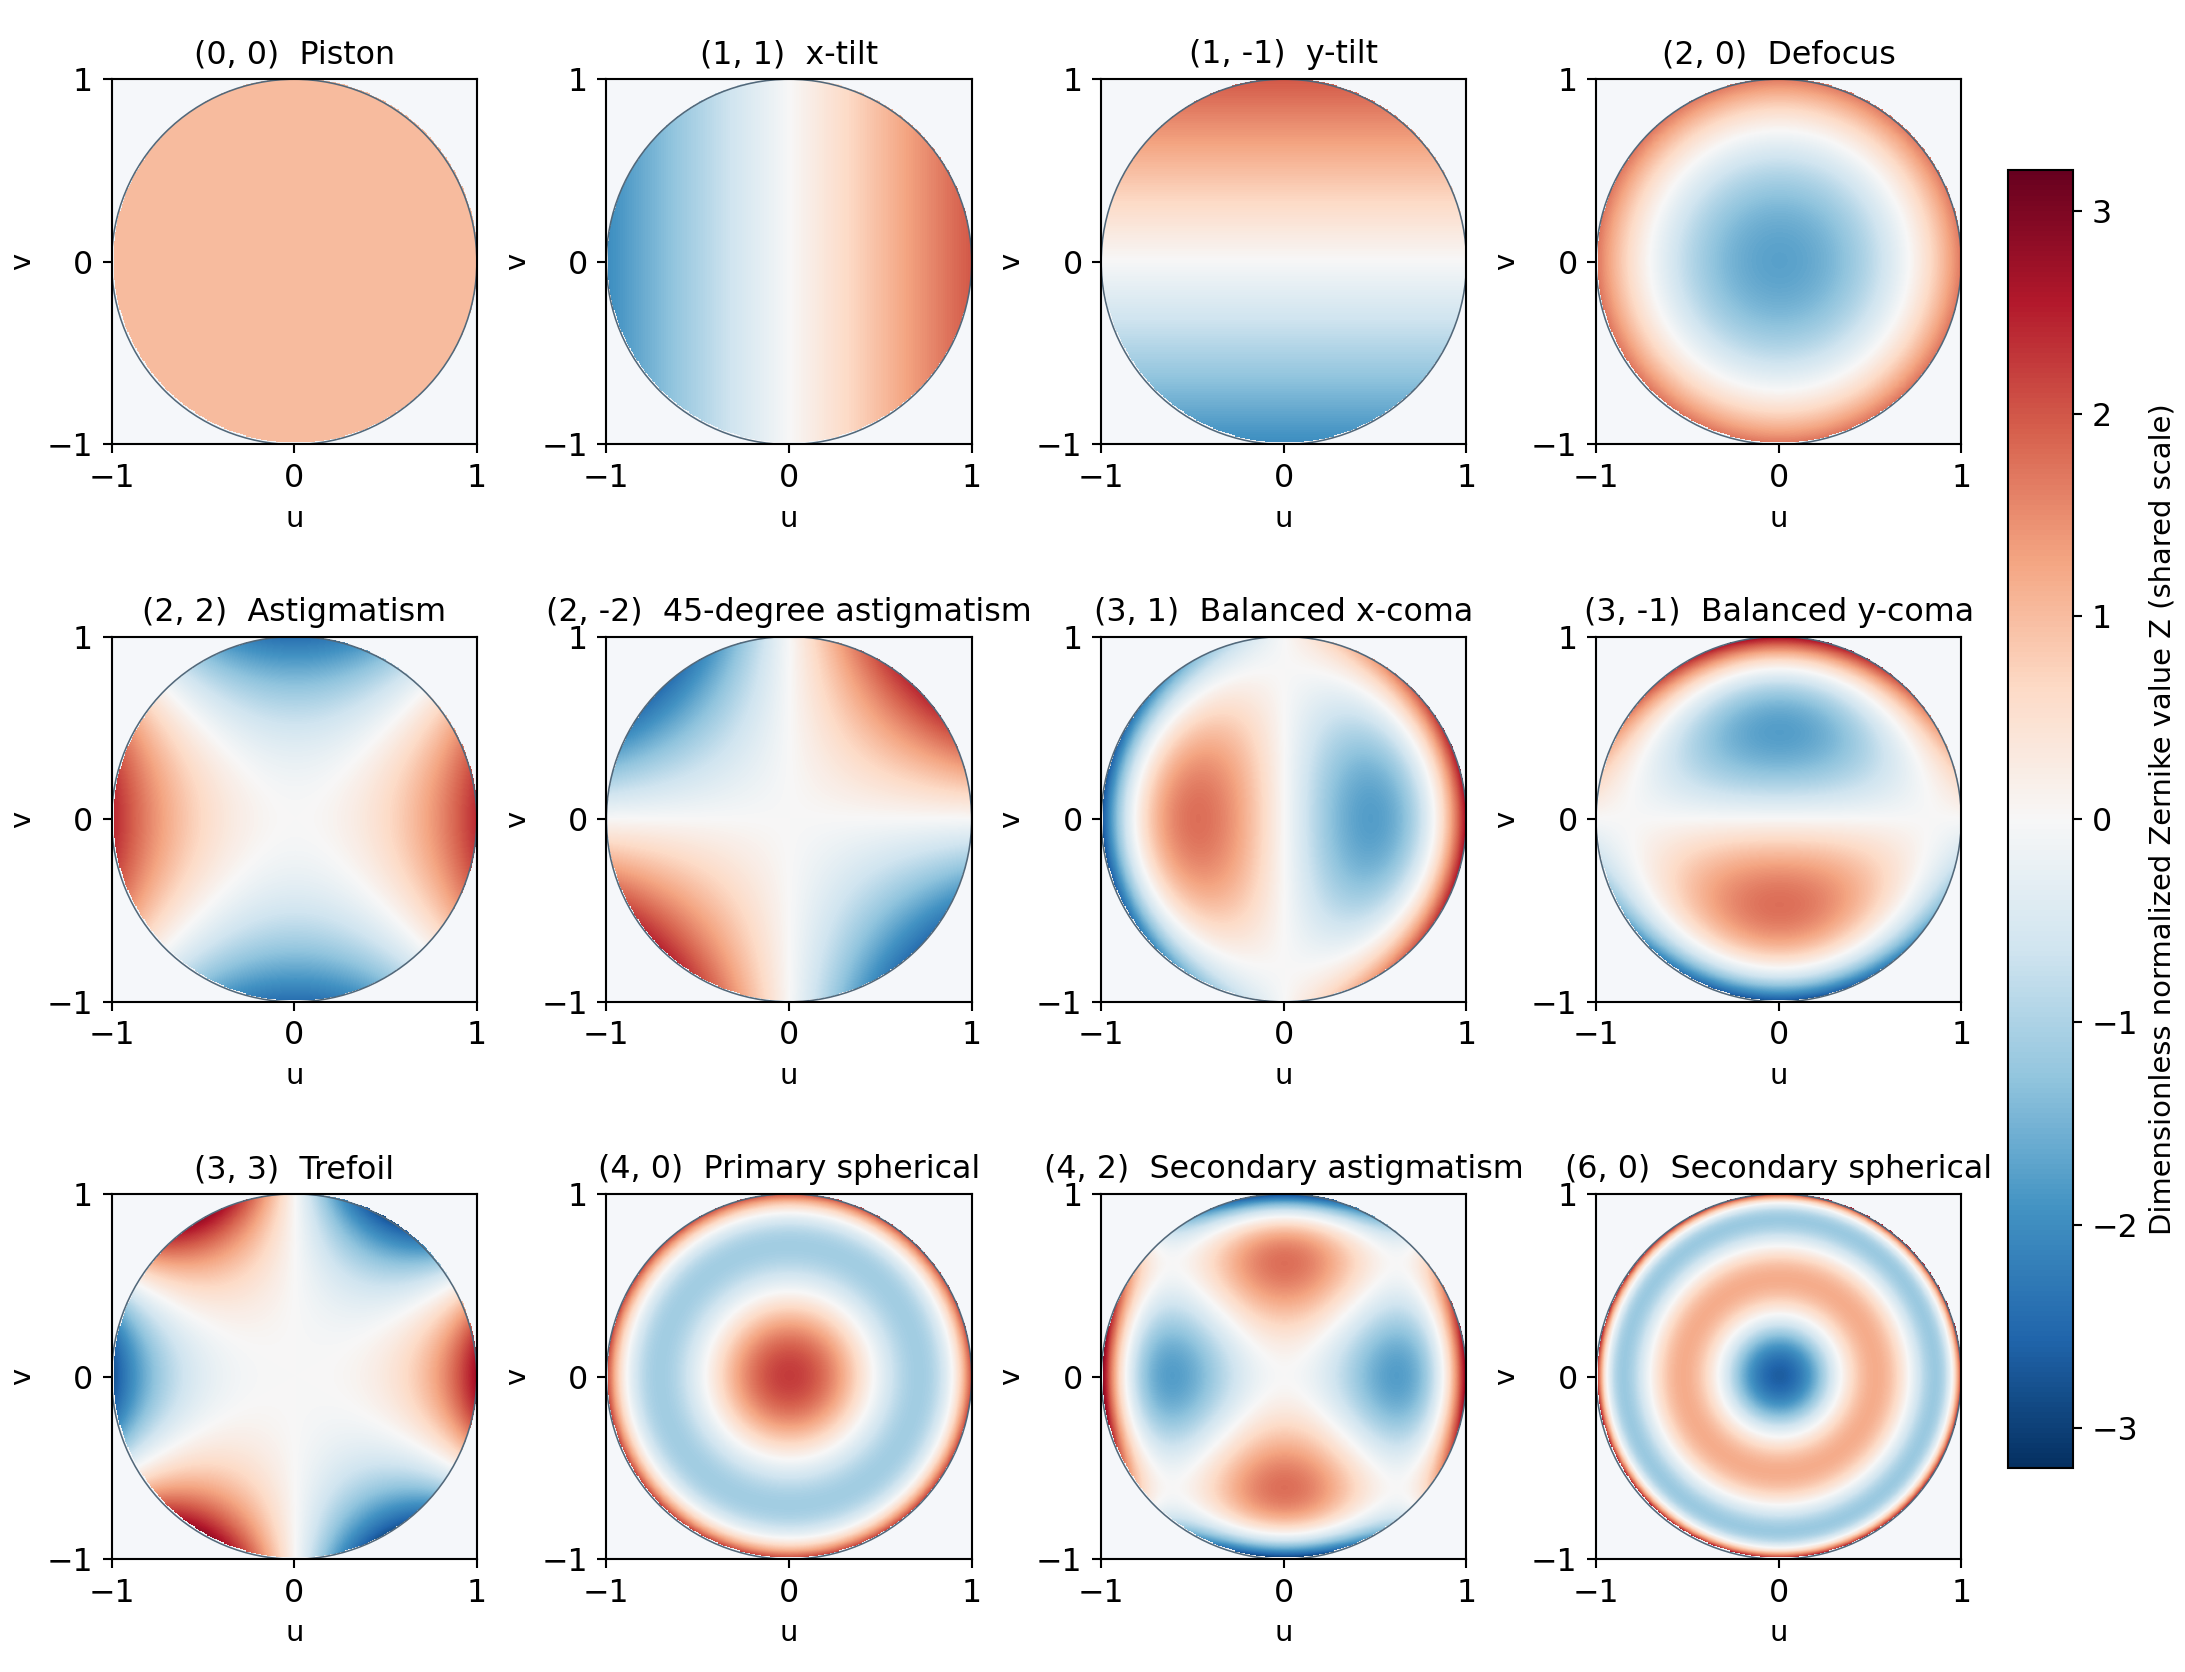
\includegraphics[width=.98\textwidth]{figures/zernike_atlas.png}
\caption{Zernike pupil-map atlas: the 12 selected modes in the supplied explanation, in the same three-row, four-column order. The labels are $(n,m)$, not a single-index numbering scheme. The numerical colour bar runs from $-3.2$ to $+3.2$ in dimensionless normalized $Z_n^m$ values, with zero at white. These are analytic polynomials sampled on a disk; the surrounding area lies outside the pupil.}
\label{fig:atlas}
\end{figure}


\newpage
\subsection{Identification of all 12 panels: read each row left to right}
\begin{longtable}{@{}p{.10\textwidth}p{.10\textwidth}p{.29\textwidth}p{.43\textwidth}@{}}
\toprule Position & $(n,m)$ & Mode & What you see\\\midrule\endhead
R1, C1 & $(0,0)$ & Piston & One constant colour everywhere.\\
R1, C2 & $(1,1)$ & Horizontal or $x$-tilt & Blue on the left, red on the right.\\
R1, C3 & $(1,-1)$ & Vertical or $y$-tilt & Red at the top, blue at the bottom.\\
R1, C4 & $(2,0)$ & Defocus & Blue centre and red outer region.\\
R2, C1 & $(2,2)$ & Primary astigmatism, aligned with coordinate axes & Red left/right and blue top/bottom.\\
R2, C2 & $(2,-2)$ & Primary astigmatism, rotated $45^\circ$ & Alternating signs in diagonal quadrants.\\
R2, C3 & $(3,1)$ & Balanced $x$-coma & Left/right structure with a radial sign reversal.\\
R2, C4 & $(3,-1)$ & Balanced $y$-coma & The corresponding top/bottom structure.\\
R3, C1 & $(3,3)$ & Trefoil & Three red and three blue angular sectors.\\
R3, C2 & $(4,0)$ & Balanced primary spherical aberration & Red centre, blue annulus, red rim.\\
R3, C3 & $(4,2)$ & Secondary astigmatism & Astigmatic angular structure with an additional radial reversal.\\
R3, C4 & $(6,0)$ & Balanced secondary spherical aberration & Alternating concentric regions, beginning blue at the centre.\\\bottomrule
\end{longtable}
This identification follows the supplied atlas explanation. Higher radial degrees introduce additional radial structure within an angular family. The twelve selected modes are an atlas, not a complete sequence through degree six.

\textbf{Why the appearances follow from the formulas.} Tilt is proportional to $u$ or $v$. Defocus changes sign where $2\rho^2-1=0$, at $\rho=1/\sqrt2$. Astigmatism's $\cos2\theta$ or $\sin2\theta$ alternates sign four times around the rim. Coma has radial factor $\rho(3\rho^2-2)$, which reverses sign at $\rho=\sqrt{2/3}$, while its $m=1$ factor makes left/right or top/bottom lobes. Trefoil's $\cos3\theta$ produces six alternating sectors.

Primary spherical's $6\rho^4-6\rho^2+1$ has zeros at
$\rho^2=(3\pm\sqrt3)/6$ and is positive both at the centre and rim. Secondary astigmatism has $\rho^2(4\rho^2-3)$, so its extra radial reversal is at $\rho=\sqrt3/2$. Finally,
\begin{equation}
Z_6^0=\sqrt7(20\rho^6-30\rho^4+12\rho^2-1)
=\sqrt7P_3(2\rho^2-1).
\end{equation}
Its three radial zeros satisfy $\rho^2=(1-\sqrt{3/5})/2,\ 1/2,\ (1+\sqrt{3/5})/2$. The centre value is negative and the rim value positive, explaining the alternating concentric colours.

\subsection{Why raw monomials are inconvenient}
On a uniform unit disk,
\begin{equation}
(f,g)=\avg{fg}=\frac1\pi\int_0^{2\pi}\int_0^1fg\rho\dd\rho\dd\theta,
\qquad \avg{\rho^{2q}}=2\int_0^1\rho^{2q+1}\dd\rho=\frac1{q+1}.
\end{equation}
Thus $(1,\rho^2)=1/2$ and $(\rho^2,\rho^4)=1/4$: the simple powers are not orthogonal. An orthonormal basis makes the coefficients independent under this pupil-area inner product. It does not make their \emph{image effects} independent.

\subsection{Constructing familiar modes by subtracting overlaps}
\textbf{Piston and tilt.} $Z_0^0=1$. Because $\avg{u^2}=\avg{v^2}=1/4$, the normalized tilts are $Z_1^1=2u$ and $Z_1^{-1}=2v$.

\textbf{Defocus.} Subtract the mean of $\rho^2$: $\rho^2-1/2$. Its mean square is $1/3-1/4=1/12$, giving
\begin{equation}
Z_2^0=\sqrt3(2\rho^2-1).
\end{equation}
\textbf{Astigmatism.} Angular averaging makes $\rho^2\cos2\theta$ orthogonal to piston and defocus, and
$\avg{\rho^4\cos^22\theta}=\tfrac12\cdot\tfrac13=1/6$. Therefore
\begin{equation}
Z_2^2=\sqrt6\rho^2\cos2\theta=\sqrt6(u^2-v^2),\qquad
Z_2^{-2}=\sqrt6\rho^2\sin2\theta=2\sqrt6uv.
\end{equation}
\textbf{Coma.} Start from $(\rho^3-b\rho)\cos\theta$ and remove its tilt overlap:
\begin{equation}
0=\avg{(\rho^3-b\rho)\rho\cos^2\theta}
=\frac12\left(\frac13-\frac b2\right),\qquad b=\frac23.
\end{equation}
Multiplying the radial factor by three makes its rim value one. Its real-mode norm is $1/8$, so
\begin{equation}
Z_3^1=\sqrt8(3\rho^3-2\rho)\cos\theta
=\sqrt8(3u\rho^2-2u).
\end{equation}
\textbf{Spherical aberration.} Orthogonalize $\rho^4+b\rho^2+c$ to $1$ and $\rho^2$:
\begin{equation}
\frac13+\frac b2+c=0,\qquad
\frac14+\frac b3+\frac c2=0
\quad\Longrightarrow\quad b=-1,\ c=\frac16.
\end{equation}
Rim normalization and unit mean square give
\begin{equation}
Z_4^0=\sqrt5(6\rho^4-6\rho^2+1).
\end{equation}
The lower-order terms in balanced coma and spherical aberration enforce orthogonality; they are not accidental corrections to an otherwise pure monomial.

\subsection{Deriving the selection rules from integer-order polynomials}
The starting requirement is a real, single-valued wavefront expanded in ordinary Cartesian polynomials $u^pv^q$, with nonnegative integer powers. Angular periodicity alone requires integer Fourier order: $\ee^{\ii m(\theta+2\pi)}=\ee^{\ii m\theta}$ implies $m\in\mathbb Z$. Polynomial regularity at the pupil centre imposes the additional radial restrictions.

Define $z=u+\ii v=\rho\ee^{\ii\theta}$ and $\bar z=u-\ii v=\rho\ee^{-\ii\theta}$. Since $u=(z+\bar z)/2$ and $v=(z-\bar z)/(2\ii)$, these variables span the same polynomial space. A homogeneous term of total degree $n$ can be written as a linear combination of
\begin{equation}
z^p\bar z^q=\rho^{p+q}\ee^{\ii(p-q)\theta},\qquad
p,q\in\{0,1,2,\ldots\},\quad p+q=n.
\end{equation}
Its angular order is $m=p-q$. Solving for the two powers gives
\begin{equation}
p=\frac{n+m}{2},\qquad q=\frac{n-m}{2}.
\end{equation}
Both must be nonnegative integers. Hence
\begin{equation}
\boxed{|m|\leq n,\qquad n-m\ \hbox{even},\qquad
m=-n,-n+2,\ldots,n.}
\end{equation}
Because $m$ and $|m|$ have the same parity, the usual equivalent rule is $n-|m|$ even. Real and imaginary parts give $\cos(|m|\theta)$ and $\sin(|m|\theta)$; for $m=0$, the sine is identically zero, leaving only one mode. This yields $n+1$ real modes at degree $n$.

Conversely, for $M=|m|$ and $n=M+2k$, $k\geq0$,
\begin{equation}
\rho^n\ee^{\ii M\theta}
=(u+\ii v)^M(u^2+v^2)^k,
\end{equation}
which is explicitly a Cartesian polynomial. A lower radial power with the same angular order must still have degree $M+2j$, with $j$ a nonnegative integer. Therefore the full degree-$n$ radial factor at that angular order has the form
\begin{equation}
R_n^M(\rho)=\rho^M\left(a_0+a_1\rho^2+\cdots+a_k\rho^{2k}\right).
\label{eq:selectionform}
\end{equation}
Orthogonalization chooses the $a_j$; it does not invent the allowed powers. In descending order these are $\rho^n,\rho^{n-2},\ldots,\rho^M$, exactly those in the Zernike factorial formula.

For example, degree three allows $m=\pm1,\pm3$: $\rho^3\cos\theta=u(u^2+v^2)$ and $\rho^3\cos3\theta=u^3-3uv^2$ are polynomials. Degree two allows $m=0,\pm2$. The apparently integer-powered expression $\rho^2\cos\theta=u\sqrt{u^2+v^2}$ is not a Cartesian polynomial. Thus an integer radial power alone is insufficient: the angular and radial orders must satisfy the parity and bound together. Nonpolynomial angular functions can still be expanded in the complete Zernike basis; the selection rules define the polynomial basis, not a ban on other physical wavefronts.

\subsection{General definition and the Legendre connection}
Allowed indices satisfy $n\geq0$, $|m|\leq n$, and $n-|m|$ even. Put $M=|m|$ and $k=(n-M)/2$. The radial polynomial is
\begin{equation}
\boxed{R_n^M(\rho)=\sum_{j=0}^{k}
\frac{(-1)^j(n-j)!}{j!(k-j)!(M+k-j)!}\rho^{n-2j}.}
\label{eq:radial}
\end{equation}
Define the normalized real functions by
\begin{equation}
\boxed{Z_n^m=\begin{cases}
\sqrt{n+1}\,R_n^0,&m=0,\\
\sqrt{2(n+1)}\,R_n^m\cos(m\theta),&m>0,\\
\sqrt{2(n+1)}\,R_n^{|m|}\sin(|m|\theta),&m<0.
\end{cases}}
\label{eq:zdef}
\end{equation}
The parity restriction is natural for a polynomial on the disk: a factor $\rho^M\cos M\theta$ or $\rho^M\sin M\theta$ is a homogeneous Cartesian polynomial, and multiplication by powers of $\rho^2=u^2+v^2$ raises its degree by two.

Use $t=\rho^2$ and the shifted weighted Rodrigues construction
\begin{equation}
Q_k^{(M)}(t)=\frac{t^{-M}}{k!}\frac{\dd^k}{\dd t^k}
\left[t^{M+k}(t-1)^k\right],\qquad
R_{M+2k}^M(\rho)=\rho^M Q_k^{(M)}(\rho^2).
\label{eq:rodrigues}
\end{equation}
The derivative contains $t^M$, so $Q_k^{(M)}$ is a degree-$k$ polynomial, not a singular function. At $t=1$, only the term with all $k$ derivatives on $(t-1)^k$ survives, so $R_n^M(1)=1$.

For $M=0$, recall Legendre's Rodrigues formula
\begin{equation}
P_k(x)=\frac{1}{2^k k!}\frac{\dd^k}{\dd x^k}(x^2-1)^k.
\end{equation}
Set $x=2t-1$. Since $(x^2-1)^k=4^kt^k(t-1)^k$ and $\dd/\dd x=\tfrac12\dd/\dd t$, the powers of two cancel:
\begin{equation}
\boxed{R_{2k}^{0}(\rho)=P_k(2\rho^2-1).}
\end{equation}
For example $P_1(x)=x$ gives $2\rho^2-1$, while
$P_2(x)=(3x^2-1)/2$ gives $6\rho^4-6\rho^2+1$.
For general $M$, the correct extension is a Jacobi polynomial:
\begin{equation}
\boxed{R_{M+2k}^{M}(\rho)=\rho^M P_k^{(0,M)}(2\rho^2-1).}
\label{eq:jacobi}
\end{equation}
The $(0,M)$ order refers to Jacobi weight $(1-x)^0(1+x)^M$. After $x=2t-1$, this is proportional to $t^M$, exactly the weight below. Thus only the azimuthally symmetric radial family is directly a shifted Legendre family; replacing all radial factors by ordinary Legendre polynomials would be incorrect. See the linked NIST definitions and Rodrigues formulas in the source record.

\subsection{Derive the factorial formula}
Expand the Rodrigues bracket:
\begin{equation}
t^{M+k}(t-1)^k=\sum_{s=0}^k(-1)^{k-s}\binom{k}{s}t^{M+k+s}.
\end{equation}
Taking $k$ derivatives, multiplying by $t^{-M}/k!$, and then by $\rho^M$ yields
\begin{equation}
R_{M+2k}^M(\rho)=\sum_{s=0}^k
\frac{(-1)^{k-s}(M+k+s)!}{s!(k-s)!(M+s)!}\rho^{M+2s}.
\end{equation}
Set $j=k-s$ and $n=M+2k$ to obtain \eqref{eq:radial}. The factorial expression therefore follows from an orthogonal-polynomial construction rather than being a formula to memorize without context.

\section{Proof of general Zernike orthogonality}
\subsection{Angular orthogonality separates different azimuthal orders}
The identity $\int_0^{2\pi}\ee^{\ii q\theta}\dd\theta=2\pi\delta_{q0}$ follows by integrating the exponential for nonzero integer $q$. Resolving sines and cosines into exponentials gives, for positive integers $M,L$,
\begin{align}
\int_0^{2\pi}\cos M\theta\cos L\theta\dd\theta&=\pi\delta_{ML},\\
\int_0^{2\pi}\sin M\theta\sin L\theta\dd\theta&=\pi\delta_{ML},\\
\int_0^{2\pi}\sin M\theta\cos L\theta\dd\theta&=0.
\end{align}
A constant integrates to $2\pi$, while every nonconstant sine/cosine has zero integral. Only modes with the same angular type and frequency can have a nonzero inner product. It remains to distinguish their radial degrees.

\subsection{Radial orthogonality at fixed angular order}
Let $F_k(t)=t^{M+k}(t-1)^k$ and take $\ell<k$. Because $\rho\dd\rho=\dd t/2$,
\begin{align}
\int_0^1R_{M+2k}^M R_{M+2\ell}^M\rho\dd\rho
&=\frac12\int_0^1t^M Q_k^{(M)}Q_\ell^{(M)}\dd t\\
&=\frac{1}{2k!}\int_0^1Q_\ell^{(M)}F_k^{(k)}\dd t.
\end{align}
Integrate by parts $k$ times. Every endpoint term contains a derivative of $F_k$ of order at most $k-1$. Such derivatives vanish at both ends: $F_k$ has a zero of order $M+k\geq k$ at zero and of order $k$ at one. The integral becomes
\begin{equation}
\frac{(-1)^k}{2k!}\int_0^1
\frac{\dd^k Q_\ell^{(M)}}{\dd t^k}\,F_k(t)\dd t=0,
\end{equation}
because $Q_\ell^{(M)}$ has degree $\ell<k$. Symmetry of the inner product handles $k<\ell$. This proves orthogonality for all unequal radial degrees at fixed $M$, including the endpoints rather than merely asserting their cancellation.

\subsection{Compute the radial norm, not just the zero overlaps}
The highest coefficient of $Q_k^{(M)}$ is
\begin{equation}
A_k=\frac{(M+2k)!}{k!(M+k)!},\qquad
\frac{\dd^kQ_k^{(M)}}{\dd t^k}=k!A_k.
\end{equation}
Perform the same $k$ integrations by parts with $\ell=k$:
\begin{align}
\int_0^1[R_{M+2k}^M]^2\rho\dd\rho
&=\frac{A_k}{2}\int_0^1t^{M+k}(1-t)^k\dd t\\
&=\frac{A_k}{2}\frac{(M+k)!k!}{(M+2k+1)!}
=\boxed{\frac1{2(n+1)}}.
\end{align}
For completeness, $B(a,b)=\int_0^1t^a(1-t)^b\dd t$ obeys
$B(a,b)=b\,B(a+1,b-1)/(a+1)$ by integration by parts; iterating to
$B(a+b,0)=1/(a+b+1)$ gives $a!b!/(a+b+1)!$ for nonnegative integers.

Combining zero overlaps and the norm,
\begin{equation}
\int_0^1R_n^M R_{n'}^M\rho\dd\rho
=\frac{\delta_{nn'}}{2(n+1)}.
\end{equation}
Multiply by the angular norm and divide by pupil area $\pi$. For $m=0$, the unnormalized norm is $1/(n+1)$; for a nonzero sine/cosine it is $1/[2(n+1)]$. The square-root factors in \eqref{eq:zdef} therefore give
\begin{equation}
\boxed{\avg{Z_n^mZ_{n'}^{m'}}=\delta_{nn'}\delta_{mm'}.}
\label{eq:orth}
\end{equation}
This proves orthogonality and normalization for every allowed real mode. Completeness is a separate statement: these modes span all Cartesian polynomial restrictions on the disk, since their leading radial terms are nonzero and the lower terms form a triangular change of basis. Polynomials are dense in the disk's $L^2$ space, so the full mode family is complete there. A finite truncation retains only its corresponding polynomial subspace.

\section{Typical aberrations in Zernike form}
\begin{center}\small
\begin{tabularx}{\textwidth}{@{}l l Y@{}}\toprule
Name & Mode & Normalized polynomial\\\midrule
Piston & $(0,0)$ & $1$\\
$x,y$ tilt & $(1,\pm1)$ & $2\rho\cos\theta$, $2\rho\sin\theta$\\
Defocus & $(2,0)$ & $\sqrt3(2\rho^2-1)$\\
Astigmatism & $(2,\pm2)$ & $\sqrt6\rho^2\cos2\theta$, $\sqrt6\rho^2\sin2\theta$\\
Balanced coma & $(3,\pm1)$ & $\sqrt8(3\rho^3-2\rho)\{\cos\theta,\sin\theta\}$\\
Trefoil & $(3,\pm3)$ & $\sqrt8\rho^3\{\cos3\theta,\sin3\theta\}$\\
Balanced spherical & $(4,0)$ & $\sqrt5(6\rho^4-6\rho^2+1)$\\
Secondary astigmatism & $(4,\pm2)$ & $\sqrt{10}(4\rho^4-3\rho^2)\{\cos2\theta,\sin2\theta\}$\\
Quadrafoil & $(4,\pm4)$ & $\sqrt{10}\rho^4\{\cos4\theta,\sin4\theta\}$\\\bottomrule
\end{tabularx}\end{center}
Here $\pm m$ means cosine first, sine second. Trefoil and quadrafoil are useful pupil modes but are not additional members of the five centred-system Seidel families in \eqref{eq:seidel}.

\subsection{Convert raw Seidel monomials into balanced modes}
Direct rearrangement of the preceding polynomials gives
\begin{align}
u&=\tfrac12 Z_1^1,&
\rho^2&=\tfrac12 Z_0^0+\tfrac1{2\sqrt3}Z_2^0,\\
u\rho^2&=\tfrac13 Z_1^1+\tfrac1{3\sqrt8}Z_3^1,&
\rho^4&=\tfrac13 Z_0^0+\tfrac1{2\sqrt3}Z_2^0+\tfrac1{6\sqrt5}Z_4^0,\\
u^2&=\tfrac14 Z_0^0+\tfrac1{4\sqrt3}Z_2^0+\tfrac1{2\sqrt6}Z_2^2.
\end{align}
In these lines $u$ is the Cartesian pupil coordinate (not a spatial frequency). Therefore $A\rho^4$ includes piston and defocus as well as balanced spherical; $Bh\,u\rho^2$ includes tilt as well as balanced coma; $Ch^2u^2$ includes defocus and piston as well as balanced astigmatism. Field curvature is a field-dependent defocus coefficient; distortion is a field-dependent tilt coefficient. They do not require special new local Zernike shapes.

\subsection{Use the same slope rule on balanced modes}
For $W=cZ_n^m$ and dimensionless image coordinate $\mathbf s=\NA\mathbf x/\lambda_0$, the ray displacement is $(c/\lambda_0)\nabla Z_n^m$. Explicit examples are
\begin{align}
\nabla Z_1^1&=(2,0),&
\nabla Z_2^0&=4\sqrt3(u,v),\\
\nabla Z_2^2&=2\sqrt6(u,-v),&
\nabla Z_2^{-2}&=2\sqrt6(v,u),\\
\nabla Z_3^1&=\sqrt8(9u^2+3v^2-2,6uv),\\
\nabla Z_4^0&=12\sqrt5(2\rho^2-1)(u,v).
\end{align}
These are the analytic gradients used in the ray panels. They make the subtraction of tilt/defocus visible as a change of ray position or focal setting, rather than a change in the diffraction law.

\subsection{Coefficients, RMS, and what balancing means}
Expand $W=\sum c_n^mZ_n^m$. Multiply by one mode and apply \eqref{eq:orth}:
\begin{equation}
\boxed{c_n^m=\avg{WZ_n^m},\qquad
\avg W=c_0^0,\qquad
\sigma_W^2=\sum_{(n,m)\ne(0,0)}(c_n^m)^2.}
\end{equation}
For a finite projection, add the residual mean square if it has not been represented; it is orthogonal to the retained modes. Other deliberately removed modes must also be excluded from the quoted residual RMS. These relations assume the full uniformly weighted disk and the stated normalization.

For raw spherical error $A\rho^4$, allow a compensating $d\rho^2$ and then remove piston. The variance is
\begin{equation}
V(d)=\frac{4A^2}{45}+\frac{d^2}{12}+\frac{Ad}{6}.
\end{equation}
Since $V'(d)=(d+A)/6$, the minimum occurs at $d=-A$. The balanced residual is
\begin{equation}
W_{\rm bal}=A(\rho^4-\rho^2+1/6)=\frac{A}{6\sqrt5}Z_4^0,
\qquad \sigma_{\rm bal}=\frac{|A|}{\sqrt{180}}.
\end{equation}
This is four times smaller than the piston-removed RMS of raw $A\rho^4$. It is a meaningful improvement only when the compensating focus adjustment is allowed. Minimizing pupil RMS also need not optimize every image metric.

\textbf{Orientation and measurement.} A pair $c_c\cos M\theta+c_s\sin M\theta$ equals
$C\cos[M(\theta-\theta_0)]$, where $C=\sqrt{c_c^2+c_s^2}$ and
$\theta_0=\operatorname{atan2}(c_s,c_c)/M$. The orientation changes under axis rotation; the pair's norm does not. For obscured pupils or nonuniform weights, the Gram matrix is generally not the identity. Sampled fitting solves
$(B^TQB)\mathbf c=B^TQ\mathbf w$, preferably using QR/SVD numerically; simply summing squared exported coefficients is then not automatically the physical RMS.

Finally, a single index such as $Z_{20}$ is not a unique physical name. Noll, Fringe, OSA/ANSI and simulator conventions differ in order, sign, and normalization. Use $(n,m)$ and the explicit polynomial to make these notes reproducible.


\appendix
\section{Supporting details: read the atlas one panel at a time}
These explanations condense the final response in the shared conversation. They supplement the main derivations; each refers to the panel positions in Fig.~\ref{fig:atlas}. The maps show $Z$ itself. A physical contribution is $W=cZ$, and a negative $c$ reverses every sign/colour stated below.

\subsection*{Row 1, column 1: piston, $(0,0)$}
$Z_0^0=1$ everywhere, so the entire disk has one constant positive colour. It has unit mean square as a basis function but zero mean-subtracted RMS. Multiplying by $c$ adds the common phase $\ee^{\ii k_0c}$ to the whole field, leaving all relative phases and the intensity unchanged. A uniformly coloured map therefore need not imply an image defect.

\subsection*{Row 1, columns 2 and 3: horizontal and vertical tilt}
$Z_1^1=2u$ is negative on the left, zero on the vertical diameter, and positive on the right. Hence blue--white--red runs horizontally. For $Z_1^{-1}=2v$, the upper half is positive, the lower half negative, and the horizontal diameter is zero. The gradient is constant, so these maps shift a point image without altering its shape. A cosine-to-sine tilt rotation is $90^\circ$.

\subsection*{Row 1, column 4: defocus, $(2,0)$}
For $Z_2^0=\sqrt3(2\rho^2-1)$, the centre is $-\sqrt3$, the rim is $+\sqrt3$, and the zero ring solves $2\rho^2-1=0$, or $\rho=1/\sqrt2\simeq0.707$. Thus blue occupies the centre and red the outer region. The white ring is a zero-OPD contour on the pupil, not a dark ring in a point image. The quadratic term describes a focus mismatch; the constant subtraction makes the pupil mean zero.

\subsection*{Row 2, column 1: axis-aligned primary astigmatism, $(2,2)$}
$Z_2^2=\sqrt6(u^2-v^2)$. On the horizontal axis $v=0$, so the value is positive; on the vertical axis $u=0$, it is negative. The zero lines are $u=\pm v$, producing diagonal white boundaries between the lobes. The two pupil directions have opposite curvature changes and different directional foci. The four-lobed pupil map is not a prediction of a four-lobed geometrical image.

\subsection*{Row 2, column 2: rotated primary astigmatism, $(2,-2)$}
$Z_2^{-2}=2\sqrt6uv$. Upper-right and lower-left quadrants have $uv>0$ and are red; upper-left and lower-right have $uv<0$ and are blue. Both coordinate axes are zero lines. The equality
$\cos[2(\theta-45^\circ)]=\sin2\theta$ shows that this is the previous angular pattern physically rotated by $45^\circ$.

\subsection*{Row 2, column 3: balanced horizontal coma, $(3,1)$}
$Z_3^1=\sqrt8\,u(3\rho^2-2)$. Its sign depends on both $u$ and radius. The radial factor changes sign at $\rho=\sqrt{2/3}\simeq0.816$. On the right ($u>0$), the inner region is negative and the outer crescent positive; on the left the signs reverse. The vertical diameter is also a zero line. The $-2u$ contribution subtracts tilt, making the mode orthogonal to $Z_1^1$. It is this balancing that produces the radial reversal absent from the raw $u\rho^2$ monomial.

\subsection*{Row 2, column 4: balanced vertical coma, $(3,-1)$}
Replace $u$ with $v$: $Z_3^{-1}=\sqrt8\,v(3\rho^2-2)$. The same radial zero remains at $\sqrt{2/3}$. Above the centre, the inner region is negative and the outer region positive; below it, these signs reverse. The horizontal diameter is a zero line. This is the same coma family with a $90^\circ$ change in orientation, not a different radial aberration.

\subsection*{Row 3, column 1: trefoil, $(3,3)$}
$Z_3^3=\sqrt8\rho^3\cos3\theta$. During one revolution, $3\theta$ runs through three cosine cycles, producing three positive and three negative sectors. The zeros are the six rays $\theta=\pi/6+j\pi/3$; the $\rho^3$ factor suppresses the magnitude near the centre and enhances it near the rim. The omitted sine partner is the same pattern rotated by $30^\circ$, because $3\times30^\circ=90^\circ$.

\subsection*{Row 3, column 2: balanced primary spherical, $(4,0)$}
$Z_4^0=\sqrt5(6\rho^4-6\rho^2+1)$ has no angular dependence. It is $+\sqrt5$ at both centre and rim, but $-\sqrt5/2$ at $\rho=1/\sqrt2$. Hence the red centre, blue annulus, and red rim. Its two zero circles follow from $6t^2-6t+1=0$, $t=\rho^2$:
\begin{equation}
\rho=\sqrt{\frac{3-\sqrt3}{6}}\simeq0.460,
\qquad \rho=\sqrt{\frac{3+\sqrt3}{6}}\simeq0.888.
\end{equation}
The quadratic and constant terms are the defocus/piston balance. This is not the monotonically increasing raw quartic $\rho^4$.

\subsection*{Row 3, column 3: secondary astigmatism, $(4,2)$}
$Z_4^2=\sqrt{10}\rho^2(4\rho^2-3)\cos2\theta$. The angular factor has the same four-sector pattern as primary astigmatism. The extra radial factor changes sign at $\rho=\sqrt3/2\simeq0.866$, reversing each angular lobe across that circle. For example, along the positive horizontal axis the inner region is negative and the rim positive. The origin is zero, but is a point rather than an interior zero circle.

\subsection*{Row 3, column 4: balanced secondary spherical, $(6,0)$}
$Z_6^0=\sqrt7(20\rho^6-30\rho^4+12\rho^2-1)$ begins at $-\sqrt7$ and ends at $+\sqrt7$. Its three interior radial zeros occur at approximately $\rho=0.336,\ 0.707,\ 0.942$. Thus its concentric regions alternate blue--red--blue--red from centre to rim. Compared with primary spherical, its higher radial degree introduces one further reversal while retaining rotational symmetry.

% \subsection*{A general reading rule and the role of normalization}
% For standard $R_n^{|m|}$, the number of interior radial zero circles is
% $(n-|m|)/2$. This follows from the $k$ simple interior zeros of the degree-$k$ Jacobi polynomial under its positive weight. Zeros at the origin from $\rho^{|m|}$ are not counted as circles. Angular sine/cosine factors separately determine the sector boundaries.

% Equal mean square does not mean equal extrema: piston is $1$, tilt reaches $2$, and primary spherical reaches $\sqrt5$. The atlas uses a common dimensionless colour bar so these differences remain visible. A physical OPD scale in nanometres requires the coefficient $c$; the map alone does not specify that coefficient.

\subsection*{Orientation: rotating a pattern versus rotating the axes}
For a normalized pair with the same $n$ and $M>0$, factor out
$F(\rho)=\sqrt{2(n+1)}R_n^M(\rho)$:
\begin{equation}
W_{\rm pair}=F(\rho)[c_c\cos M\theta+c_s\sin M\theta]
=CF(\rho)\cos[M(\theta-\theta_0)].
\end{equation}
Expanding the cosine of a difference gives
$c_c=C\cos M\theta_0$, $c_s=C\sin M\theta_0$, hence
\begin{equation}
C=\sqrt{c_c^2+c_s^2},\qquad
\theta_0=\frac{\operatorname{atan2}(c_s,c_c)}{M}.
\end{equation}
The pair's RMS is $C$ by orthonormality; orientation is undefined if $C=0$. For astigmatism coefficients $(0.03,0.04)\,\mathrm{nm}$, $C=0.05\,\mathrm{nm}$ and $\theta_0=53.13^\circ/2=26.565^\circ$.

If the coordinate axes rotate counterclockwise by $\alpha$, then
$\theta=\theta'+\alpha$, and collecting the new sine/cosine terms gives
\begin{equation}
\begin{pmatrix}c_c'\\c_s'\end{pmatrix}
=\begin{pmatrix}\cos M\alpha&\sin M\alpha\\-\sin M\alpha&\cos M\alpha\end{pmatrix}
\begin{pmatrix}c_c\\c_s\end{pmatrix}.
\end{equation}
For $M=2$, $\alpha=45^\circ$, this is $(c_c',c_s')=(c_s,-c_c)$. In contrast, physically rotating a cosine astigmatism pattern by $45^\circ$ while holding the axes fixed produces the \emph{positive} sine partner. Changing coordinates consistently changes no physics; rotating the aberration relative to a fixed mask/illumination can change imaging while preserving RMS.


% \section{Source map and reproducibility}
% \subsection*{Sources actually used}
% \begin{enumerate}
% \item \textbf{Supplied local textbook,} \emph{Understanding the Aberration Budget Paper}: Chapter 5, printed pp.~22--25 (PDF pp.~31--34); Chapter 6, printed pp.~27--29 (PDF pp.~36--38); Chapter 7, printed pp.~30--35 (PDF pp.~39--44). The Rodrigues proof also uses Appendix A.1, printed pp.~81--82 (PDF pp.~90--91). The local source file is \texttt{aberration\_budget\_textbook.pdf} under \texttt{aberration budget paper}.
% \item \textbf{Shared conversation,} \href{https://chatgpt.com/share/6ad705f0-b784-83ec-bca0-9933ba39540c}{\emph{Stepwise Optics Derivation Explanation}}, recovered 20 October 2026. Used the response on textbook Sections 6.2--6.4, especially its numbered points 6--14; its original pupil/image HTML; the final response's 12-panel explanation, rotation discussion, and balancing discussion; and its selection-rule and Legendre/Jacobi explanations. Relevant extracted text and original visualization data are retained under \texttt{checks/}.
% \item \textbf{User-supplied screenshots,} the original eleven mathematical extracts plus the later 12-panel identification table. The three interface sections and polarization derivations retain the requested subdivision.
% \item \textbf{Independent mathematical reference:} NIST Digital Library of Mathematical Functions, \href{https://dlmf.nist.gov/18.3}{\S18.3, Definitions} and \href{https://dlmf.nist.gov/18.5}{\S18.5, Explicit Representations}. Used to cross-check the Jacobi/Legendre convention; the orthogonality proof is written out in these notes.
% \item \textbf{Independent interface reference:} MIT OpenCourseWare, \href{https://www.ocw.mit.edu/courses/6-974-fundamentals-of-photonics-quantum-electronics-spring-2006/fafcb9e36b7749f4eeb099d666bdf70a_electr_wav_inter.pdf}{\emph{Electromagnetic Waves and Interfaces}}, \S2.2. Used to cross-check the boundary/phase-matching framework; our displayed amplitude and time conventions are explicitly stated.
% \end{enumerate}

% \subsection*{Requested flow: coverage record}
% \begin{tabularx}{\textwidth}{@{}lY@{}}\toprule
% Requested material & Placement / treatment\\\midrule
% Complex optical constant & Section 1: decay, relative material phase, and limitations of black paint.\\
% Photos 1--3; photo 7 & Section 2: separate electric continuity, magnetic sign, solution for $r,t$; Snell's law is the boundary-condition side discovery.\\
% Photos 4--6; photo 9 & Section 3: polarization-specific derivations; reverse-interface identities are proved earlier in Section 2.\\
% Photos 8 and 10 & Sections 4--5: geometric series and bottom-up multilayer recursion.\\
% Photo 11; chat points 6--14 & Sections 6--7: Fresnel cancellation, ray gradients, all five classical families, field dependence, and general piston invariance.\\
% Original HTML illustration & \texttt{aberration\_illustration.html}: original stored data with added polar and Zernike formulas.\\
% Adjustable companion HTML & \texttt{aberration\_explorer.html}: coefficient/field/focus controls, ray diagrams, FFT images, and atlas.\\
% Small-error RMS and degeneracy & Section 9: brief expansion with fixed-point/peak distinctions and nonuniqueness examples.\\
% Zernike plots and detailed explanation & Section 10: atlas and supplied identification table; Appendix A: supplementary panel-by-panel commentary from the final chat response.\\
% Selection rules, Legendre, orthogonality & Sections 10--11: Cartesian polynomial derivation, Jacobi generalization, and full endpoint/norm proof.\\
% Typical Zernike aberrations & Section 12: normalized formulas, raw-to-balanced decomposition, slopes, and RMS.\\\bottomrule
% \end{tabularx}

% \subsection*{How to rerun or edit}
% Edit \texttt{study\_notes\_20\_oct.tex} and its \texttt{sections/} files. Run \texttt{build\_notes.ps1} to check the calculations, regenerate figures, and compile with the existing workspace Python and MiKTeX; SyncTeX is enabled and every figure uses \texttt{[H]}.

% Open \texttt{optics\_demonstrations.ipynb} in Jupyter or VS Code. Edit the parameter cell and run the later cells. Keep the imported \texttt{optics\_calculations.py} beside it. Defaults are teaching examples, not measured materials or a scanner reconstruction.

% The Python verifier checks film series/limits, recursion against characteristic matrices, power conservation, exact polynomial identities, the Gram matrix through degree eight, and Fourier piston/tilt behaviour. The JavaScript verifier checks HTML formulas, gradients, FFT invariants, and preservation of the original seven-case data. Results, source extracts, and hashes are under \texttt{checks/}; \texttt{README.txt} gives commands and dependencies.

% \textbf{Numerical checks within the stated model.} The 320 stack comparisons agreed within $3.6\times10^{-16}$ in complex amplitude; the 45-mode Gram matrix through $n=8$ agreed with identity within $3.7\times10^{-14}$.

\end{document}
